%
% File: chap01.tex
% Author: Victor F. Brena-Medina
% Description: Introduction chapter where the biology goes.
%

\selectlanguage{spanish}
\let\textcircled=\pgftextcircled
\chapter{Introducci\'on}
\label{chap:intro}

En este capítulo se describen el contexto, la problemática a resolver, los objetivos, los retos enfrentados durante el desarrollo del proyecto y el impacto socioeconómico que tiene este trabajo de tesis. Asimismo, se detalla la organización del documento.

\section{Contexto}
\label{sec:sec01}

%\initial{H}
Hoy en d\'ia, el t\'ermino Big Data ha resonado en gran parte de los sectores econ\'omicos, sociales y laborales, provocando una ardua b\'usqueda por manipular y aprovechar la inmensa cantidad de datos que se encuentran circulando en la nube de Internet. Los datos al provenir directamente de los usuarios, a trav\'es de una gran variedad de medios digitales como las redes sociales, smartphones, sitios web, entre otros, se convierten en datos potencialmente de inter\'es para todo aquel involucrado en la b\'usqueda de soluciones dirigidas a problem\'aticas estad\'isticas, predictivas, anal\'iticas, entre otras.

%=======
\section{Problem\'atica}
\label{sec:sec02}

Una de las problemáticas que ha surgido en las organizaciones involucradas en el sector de Ingenier\'ia de Software, es encontrar candidatos con cierto tipo de habilidades, conocimientos o experiencia en el desarrollo de software, ya que a trav\'es de medios tradicionales como curr\'iculums vitae (CV), solicitudes de trabajo impresas o  incluso, mediante buscadores de Internet como Google o los propios motores de b\'usqueda que implementan los sitios web, es necesario invertir mucho tiempo, pues generalmente, las búsquedas son realizadas contemplando el contenido completo de las páginas o sitios web, mostrando resultados que pueden o no acercarse a lo que el interesado requiere. 

Por ello, es necesario desarrollar herramientas que permitan realizar búsquedas más específicas a comparación de las que actualmente existen, de manera que agilicen el proceso de análisis al efectuar una consulta dirigida a cierto subconjunto del contenido completo de datos  a examinar.

En este caso, si se requiere buscar perfiles con cierto tipo de habilidades y experiencia en un área, al realizar la búsqueda analizando campos específicos en páginas web, mostraría resultados con mayor valor para las organizaciones, puesto que la información obtenida sería más asertiva en cuanto a la consulta.

Por lo anterior, se plantea la propuesta de implementar un sistema enfocado en procesar perfiles p\'ublicos relacionados al sector de Ingenier\'ia de Software, ambiente donde los candidatos generalmente mantienen su informaci\'on laboral, personal, y en ocasiones, sus conocimientos pr\'acticos en el desarrollo de software dentro de diversos sitios web.


\section{Objetivos}
\label{sec:sec03}

\subsection{General}
\label{subsec:subsec03}

Desarrollar un sistema de b\'usqueda que permita encontrar perfiles de usuario en el sector de Ingenier\'ia de Software, utilizando t\'ecnicas y herramientas Big Data para la extracci\'on, transformaci\'on, limpieza, almacenamiento, procesamiento y an\'alisis de los datos.

\subsection{Espec\'ificos}
\label{subsec:subsec03}
  \begin{itemize}
	\item Definir el modelo del proceso de an\'alisis de datos que nos permita implementar nuestra herramienta.

	\item Seleccionar las fuentes de datos que sean de inter\'es para la soluci\'on planteada.

	\item Extraer los datos a trav\'es de las APIs disponibles para cada uno de los sitios web (LinkedIn, GitHub, Twitter).

	\item Evaluar las tecnolog\'ias para realizar b\'usquedas de texto (Elasticsearch y Solr).

	\item Analizar y evaluar el algoritmo de búsqueda de texto implementado por la tecnología elegida.
    
	\item Evaluar los resultados obtenidos a las consultas.
    \item Implementar el sistema de búsqueda. 
\end{itemize}

%=======

\section{Retos durante el proyecto}
\label{sec:sec04}

El primer obstáculo al que nos enfrentamos durante el desarrollo del proyecto fue encontrarse con ciertas limitantes de acceso a la información en cada una de las APIs constituidas en las redes sociales seleccionadas. Ya que al encontrarnos en un momento en donde las actualizaciones de los sitios web son esenciales, nos involucramos en una carrera contra tiempo, en donde las mejoras a los sitios web están a la orden del día, lo que nos lleva a la posibilidad de enfrentarnos a la problemática del acceso a los datos de los perfiles. Tal y como ocurrió en nuestro caso, pues al tratar de manipular el API de LinkedIn, ésta sufrió algunas modificaciones realizadas por la organización propietaria y como resultado surge la restricción de acceso a la información de los perfiles.

Asimismo, debido a la existencia de una gran variedad de tecnologías Big Data, el siguiente obstáculo aparece al momento de elegir aquella tecnología que se adapte mejor a la necesidad de solucionar la problemática que nos concierne. 

Una vez seleccionadas las tecnologías para implementar el sistema, nos enfrentamos a la curva de aprendizaje ante ellas, lo que implica invertir tiempo en la familiarización del flujo de trabajo de cada tecnología. 

Uno de los retos significativos surgió durante la implementación de la tecnología Elasticsearch, la cual, al ser la encargada del análisis y búsqueda de datos, fue necesario realizar algunas modificaciones en el esquema de almacenamiento de los documentos con la información pertinente de los usuarios.


%=======

\section{Impacto socioecon\'omico}
\label{sec:sec05}

\subsection{Agilizar la búsqueda de perfiles involucrados en el sector de Ingeniería de Software}
\label{subsec:subsec05}

Como se menciona en la problemática de la investigación, la búsqueda a través de medios tradicionales involucra mayor atención y tiempo de los interesados, debido al hecho de requerir la verificación de datos de los candidatos obtenidos de las consultas realizadas.

Por ello, el sistema SOFTSE al acceder directamente en el campo donde se encuentra la información de interés sobre la consulta, disminuye la cantidad de tiempo y recursos invertidos por los interesados, además de incrementar la precisión en la recuperación de los datos.

\subsection{Aumento de la precisión al obtener los datos}
\label{subsec:subsec05}

Los perfiles al ser analizados únicamente por el campo donde se encuentran los datos de interés, permite obtener mayor precisión al momento de realizar las búsquedas dentro de los campos específicos.

\subsection{Ayuda en la toma de decisiones al momento de elegir un candidato}
\label{subsec:subsec05}

Puesto que el sistema analiza los perfiles conforme a un campo específico de toda la información, y despliega los resultados en orden de relevancia al peso obtenido por campo, los resultados obtenidos facilitan la toma de decisiones al momento de seleccionar los perfiles de candidatos que tienen mayor coincidencia con la consulta realizada.

\subsection{Organización del documento}
\label{subsec:subsec06}
Esta investigaci\'on está organizada en siete cap\'itulos, distribuidos de la siguiente manera:

Cap\'itulo 1:  \textit{Introducci\'on}, establece el contexto y los aspectos relacionados a la soluci\'on de la problem\'atica de la investigaci\'on.

Cap\'itulo 2: \textit{Marco Te\'orico}, se presentan todos los planteamientos te\'oricos involucrados sobre la problem\'atica de la investigaci\'on.

Cap\'itulo 3: \textit{Antecedentes}, brinda referencia a informaci\'on de estudios realizados, relacionados con la investigaci\'on.

Cap\'itulo 4: \textit{Metodología del Proyecto}, presenta el proceso llevado a cabo para la implementaci\'on de la soluci\'on.

Cap\'itulo 5: \textit{SOFTSE}, describe el sistema de búsqueda desarrollado.

Cap\'itulo 6: \textit{Evaluación y Resultados}, muestra las evaluaciones realizadas para validar el sistema SOFTSE.

Cap\'itulo 7: \textit{Conclusiones y Trabajo Futuro}, se presentan conclusiones finales, así como las opciones de trabajo futuro que podrían ser implementadas para darle continuidad a esta investigación.

%=========================================================

\chapter{Marco Te\'orico}
\label{chap:marco}

En este capítulo, se delimita el campo que es afectado por la problemática que nos concierne. Asimismo se describen y justifican, los principales conceptos involucrados durante la investigación: Big Data, Modelo de Proceso de Análisis, las redes sociales y herramientas empleadas en el desarrollo del sistema.

\section{Big Data}
\label{sec:sec01}
%\initial{A}
A consecuencia de la aparición del Internet, y posteriormente a las redes sociales y las nuevas tecnologías del siglo XXI, se han producido cambios impresionantes tanto sociales como económicos. Debido al incremento exponencial de la cantidad de datos circulando en Internet, donde las redes sociales han jugado un papel importante en el aumento de dicha información. Tal ha sido el impacto de la enorme cantidad de datos que se menciona “\textit{nos encontramos en la era Big Data}” (\citeauthor{bigdata_art}, \citeyear{bigdata_art}).

El concepto Big Data comenzó a resonar fuertemente entre las personas familiarizadas en  las TIC’s y el análisis de datos, y aunque no existe definición única para este término, es aplicado para aquel volumen de datos variados que aumenta velozmente, que no puede ser procesado o analizado utilizando procesos o herramientas tradicionales. El principal objetivo en Big Data es analizar y procesar grandes cantidades de datos con la finalidad de producir un beneficio.

Existe más de una definición sobre este término, todo depende de cómo y dónde sea implementado por el autor.

“\textit{Big Data es información en altos volúmenes, alta velocidad o alta variedad que demanda formas creativas y viables económicamente para procesarla con el fin de contribuir a tomar decisiones, actuar y crear valor}” (\citeauthor{garner}).

“\textit{Cada día creamos 2.5 quintillones de bytes de datos, tanto que el 90\% de los datos en el mundo de hoy se han creado solamente en los últimos dos años. Este dato viene de todas partes: sensores utilizados para recabar información climática, entradas a sitios de medios sociales, fotos digitales y videos, registros de transacciones de compra y las señales de teléfono celular GPS para nombrar unos pocos. Estos datos son Big Data}” (\citeauthor{IBM}).

El término Big Data es bastante controversial, debido al desconocimiento real de su significado, inclusive desde la definición de la estrategia de implementación, el planteamiento de los objetivos o problemáticas a solucionar, la cantidad de recursos humanos y económicos, así como el nivel de experiencia ante las tecnologías sobre Big Data, y lo principal la cantidad de datos.

IBM en el año 2012, realizó una encuesta con la finalidad de determinar el significado de Big Data (\citeauthor{artBigData}, \citeyear{artBigData}), los resultados que obtuvieron se muestran en la Figura 2.1.

% A single figure
\begin{figure}[H]
	\centering
	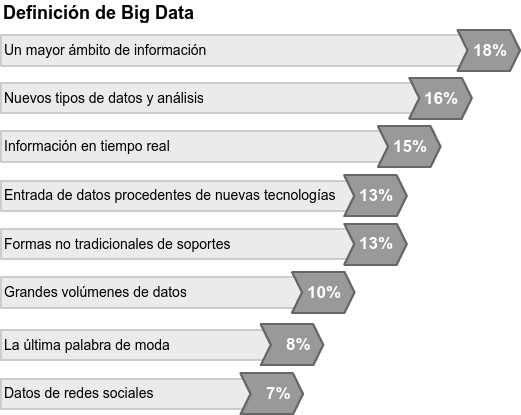
\includegraphics[height=0.3\textheight]{fig01/bigdata_enc}
	\mycaption[Resultados de la encuesta realizada por IBM.]{Resultados de la encuesta realizada por IBM (\citeauthor{artBigData}, \citeyear{artBigData}).}
	\label{fig:RHP02}
\end{figure}

Estos resultados coinciden con la forma útil para describir Big Data mediante las tres V’s (Volumen, Variedad y Velocidad)

\textbf{Volumen}. Se refiere a la cantidad de datos, y es la característica principal cuando se habla de Big Data, ya que en esencia el volumen es la diferencia de las tecnologías tradicionales al soportar la manipulación, almacenamiento y procesamiento de  la cantidad masiva de datos.

\textbf{Variedad}. Hace referencia a la manipulación de gran diversidad de tipos de datos, entre los que se encuentran los datos estructurados, semi-estructurados y no estructurados.

\textbf{Velocidad}. Es la capacidad para crear, procesar y analizar grandes cantidades de datos en tiempo real.

Algunos actores agregan otra V como parte de la definición de Big Data:

\textbf{Veracidad}. Es una característica que poco a poco ha comenzado a ser considerada como  parte de la definición de Big Data. IBM explica la veracidad como el nivel de fiabilidad asociado a los datos (\citeauthor{artBigData}, \citeyear{artBigData}). Es necesario asegurarse que la procedencia de los datos sea de fuentes confiables, de manera que el nivel de incertidumbre de los datos sea mínimo. 

\section{Modelo del Proceso de Análisis}
\label{sec:sec02}

En el mundo del análisis de Big Data, se implementa un proceso o ciclo de análisis, el cual describe las etapas requeridas para analizar datos y obtener un beneficio significativo sobre los objetivos definidos inicialmente. 

Por ello, el proceso llevado a cabo para la implementación del sistema SOFTSE, se realizó tomando como base el Modelo de Proceso de Análisis (Analytics Process Model) descrito por Baesen (\citeyear{Analytics}). En la Figura 2.2, se puede observar el Modelo de Proceso de Análisis resultante, integrado por 6 etapas representativas durante el desarrollo de nuestro sistema. 

% A single figure
\begin{figure}[H]
	\centering
	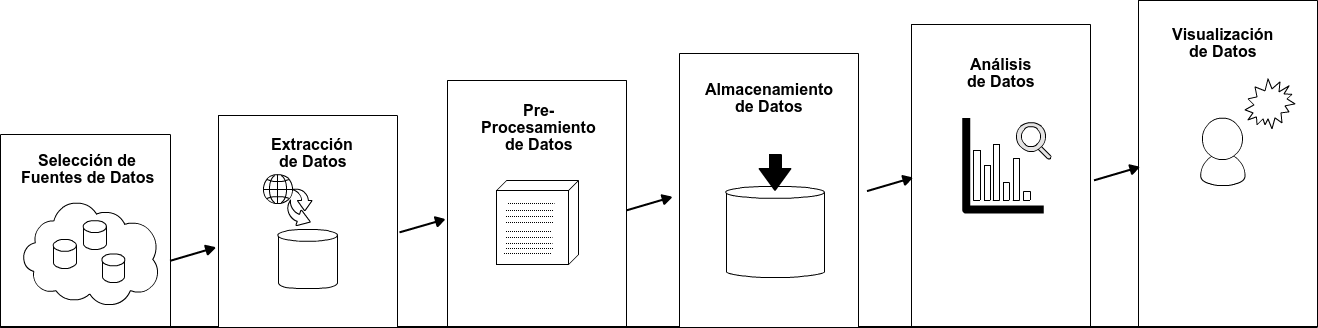
\includegraphics[height=0.17\textheight]{fig01/procesotesis.png}
	\mycaption[Modelo de Proceso de Análisis definido para la implementación del sistema \textit{SOFTSE}]{Modelo de Proceso de Análisis definido para la implementación del sistema \textit{SOFTSE}}
	\label{fig:RHP02}
\end{figure}

\textbf{Etapa 1: Selección de Fuentes de Datos.} Es importante resaltar, que antes de comenzar el proceso fue necesario definir claramente la problemática de interés a resolver mediante el análisis de los datos. Una vez definido el problema, la primer etapa consiste en identificar todos los datos fuente como datos de interés potencial, este paso es clave ya que en cualquier análisis, los datos seleccionados serán los que determinen el impacto del sistema desarrollado.

Hoy en día, existe una gran cantidad de redes sociales que permiten a sus usuarios interactuar de diferentes formas, lo anterior hace que la información de cada red social varíe y por lo tanto, fue necesario realizar una valoración del tipo de información de interés que pueden proponer algunas redes sociales como Facebook, Twitter, LinkednIn, Google+.


\textit{\textbf{Facebook}}. Red social fundada en el 2004, tiene como objetivo que la gente pueda conectarse con amigos y familiares para compartir y expresarse sobre lo que les interesa (\citeauthor{facebook_page}, \citeyear{facebook_page}).  

\textit{\textbf{Twitter}}. Red social fundada en San Francisco en 2006. Tiene más de 320 millones de usuarios activos cada mes en todo el mundo (\citeauthor{twitter_page}, \citeyear{twitter_page}), alrededor de 7000 tweets son enviados por segundo, lo cual corresponde a generar un aproximado de 600 millones de tweets por día (\citeauthor{tweets_count}, \citeyear{tweets_count}). Es una de las redes sociales más populares para compartir ideas e información en tiempo real, a través de microblogs nombrados tweets que permiten obtener información reciente sobre lo que está sucediendo (\citeauthor{twitter_page}, \citeyear{twitter_page}).

\textit{\textbf{LinkedIn}}. Desde sus inicios en 2003, LinkedIn se ha convertido en la red social más popular entre los usuarios, no sólo a nivel personal sino especialmente a nivel profesional, ya que es un servicio de redes sociales para empresas y profesionales. Está disponible en más de 200 países de todo el mundo y en 20 idiomas diferentes, permite a los miembros crear perfiles y hacer conexiones con otras personas para establecer relaciones profesionales. Actualmente, LinkedIn cuenta con más de 360 millones de usuarios activos (\citeauthor{linkedin_page}, \citeyear{linkedin_page}).


\textit{\textbf{Google+}}. Es un servicio de red social, lanzado por Google en 2011, constituye el mismo objetivo que Facebook, compartir información e interactuar con otras personas. Integra todos los servicios de Google, entre ellos su motor de búsqueda y los perfiles (\citeauthor{googleplus_page}, \citeyear{googleplus_page}).

\textit{\textbf{GitHub}}. Es el mayor host de código en el planeta, con más de 38 millones de repositorios grandes o pequeños, cada repositorio cuenta con las mismas herramientas poderosas de esta plataforma. Dichas herramientas están abiertas a la comunidad para proyectos públicos y para proyectos de inversión en el sector privado. Los usuarios tienen la posibilidad de utilizar Git o subversion como Sistema de Control de Versiones  (VCS) para administrar, mantener e implementar proyectos de software. GitHub tiene aplicaciones de escritorio para Windows, OSX y Android (\citeauthor{github_page}, \citeyear{github_page}).

Como se puede observar en la descripción de cada una de las redes sociales mencionadas anteriormente, podemos destacar a LinkedIn, Twitter y GitHub, para ser las fuentes que contienen los datos de interés en la solución de la problemática planteada. 

%========================================================
\textbf{Etapa 2: Extracción de Datos}. 
Las fuentes de datos definidas fueron tres redes sociales: LinkedIn, GitHub y Twitter, puesto que cada una proporciona datos de interés para el análisis e identificación de perfiles públicos involucrados en el sector de Ingeniería de Software. Dentro de los perfiles de sus usuarios se encuentran datos como: nombre, localización, habilidades, ocupación, áreas de conocimiento, entre otras características.

El proceso de extracción de los datos implementado para cada una de las fuentes de datos seleccionadas fue mediante el uso de APIs propias de cada plataforma.

\textit{\textbf{API GitHub}}. La plataforma de desarrollo colaborativo, GitHub, cuenta con una API para desarrolladores, la cual puede ser aprovechada mediante librerías para los distintos lenguajes de programación como Java, JavaScript, Perl, Php, Ruby, Scala, Shell, Python, entre otros (\citeauthor{ApiGit}, \citeyear{ApiGit}). 


Para utilizar el API de GitHub es requerido llevar a cabo el proceso de autenticación, con la finalidad de adquirir la autorización y los permisos para hacer ciertas operaciones u obtener acceso a recursos específicos. En el Apéndice A se incluyen las diversas maneras de autenticación para el API de GitHub. Conforme al tipo de autenticación que sea elegido dependerá el límite de peticiones que se pueden hacer, sin autenticación sólo se permiten realizar 60 peticiones por hora. La autenticación básica o OAuth, permite hacer 5,000 peticiones por hora (\citeauthor{ratelimit_github}, \citeyear{ratelimit_github}).

\textit{\textbf{X-Raying Google - LinkedIn}}. La red social LinkedIn con el objetivo de ofrecer mayor calidad a la experiencia de sus usuarios, anunció e implementó cambios significativos (\citeauthor{LinkChange}, \citeyear{LinkChange}) (\citeauthor{LinkChangeToday}, \citeyear{LinkChangeToday}), principalmente sobre sus APIs limitando el acceso a los datos de los perfiles, de tal manera que el API que llamaremos de “principiantes”, sólo permite acceder a los datos del perfil básico (nombre, apellido, industria, estatus actual, conexiones, especialidades, etc), ubicación (id, nombre) y posición laboral (título, descripción o resumen del cargo desempeñado, compañía, fecha de inicio, fecha de conclusión, posición actual, etc) (\citeauthor{LinkFields},  \citeyear{LinkFields}). Al tener acceso limitado sobre la información de los perfiles de usuario, entre los cuales se incluye la restricción a los datos de interés como las habilidades de un usuario, se opta por utilizar una técnica llamada X-Raying (\citeauthor{xgoogle}, \citeyear{xgoogle}), la cual consiste en realizar búsquedas bajo el siguiente criterio: [\textit{site:URL “texto de búsqueda”}] utilizando un motor de búsqueda, para este caso en particular se hizo uso del motor de búsqueda Google. La siguiente consulta muestra un ejemplo de búsqueda por la técnica X-Raying:
\begin{center}
\textit{site:linkedin.com/in “ingeniero de software”}
\end{center}
Al realizar X-Raying sobre Google, permite encontrar una cantidad significativa de perfiles de expertos pertenecientes al sector de Ingeniería de Software dentro de LinkedIn, que es el sector seleccionado para realizar el estudio y dar solución a la problemática que nos concierne. Se menciona que es una cantidad significativa, ya que el motor de búsqueda Google muestra los primeros 1000 resultados con un máximo de 100 por página, la cantidad de resultados se puede especificar dentro de la configuración del motor de búsqueda (\citeauthor{GooglePage}, \citeyear{GooglePage}). Al contemplar la limitante de la cantidad de resultados, se elige realizar las búsquedas por ubicación, seleccionando algunos países del Continente Americano (Argentina, Brasil, Canadá, México y Estados Unidos). Filtrar los perfiles de expertos por ubicación consiste en realizar las búsquedas conforme a los códigos de cada país (\citeauthor{countriesLink}, \citeyear{countriesLink}), de manera que el url o enlace cambiará dentro de las instrucciones de búsqueda, un ejemplo sería al momento de filtrar los perfiles de Argentina (code country: “ar”): site:ar.linkedin.com/in “ingeniero de software”, y así sucesivamente para cada uno de los países seleccionados.

\textit{¿Por qué usar Google X-Raying y no el motor de búsqueda de Linkedin?}
Si bien, el motor de búsqueda de LinkedIn tiene mayor precisión, es más potente y configurable al momento de realizar búsquedas ya que ofrece mayor control al recuperar lo que se necesita, los resultados que muestra son en base a los contactos de primer$^{1a}$ y segundo$^{1b}$ grado de la propia red de contactos, y aunque contempla los contactos de tercer$\footnote{ a) Personas con la que se está conectado directamente, b) Personas que están conectadas con los contactos de primer grado y c) Personas que están conectadas con los contactos de segundo grado (\citeauthor{red_contactos}, \citeyear{red_contactos}). }^{c}$ grado, comúnmente no permiten ver la información pública de los perfiles, es por ello que al aplicar la técnica de Google X-Raying, se puede acceder a los perfiles públicos más allá de la propia red de contactos dentro de LinkedIn, inclusive invirtiendo menor cantidad de tiempo (\citeauthor{xgooglevsLink}, \citeyear{xgooglevsLink}).

\textit{\textbf{API Twitter}}. Al igual que en GitHub, la red social Twitter también proporciona un API para desarrolladores, la cual puede ser utilizada mediante varias librerías en distintos lenguajes de programación desde ASP, C++, .NET, Java, JavaScript, Node.js, Python, Php, Ruby, entre otros (\citeauthor{ApiTwit}, \citeyear{ApiTwit}). En el Apéndice B se incluye el proceso para obtener las claves de autenticación de acceso al API de Twitter. Debido, a que ésta cuenta con un límite de 15 peticiones por ventana (\citeauthor{ratelimit_twitter}, \citeyear{ratelimit_twitter}), se decidió optar por hacer la recolección de tweets a través de la combinación de las tecnologías Elasticsearch y Logstash, puesto que de esta manera, la recolección de tweets es interna.

\textbf{\textit{Elasticsearch}}. Motor de análisis y búsqueda distribuido en tiempo real. Permite explorar datos velozmente y a gran escala. Es utilizado para realizar búsquedas full-text, estructuradas y analíticas (\citeauthor{Gormley}, \citeyear{Gormley}). Además, incorpora el análisis de \textit{logs}\footnote{Archivos que contienen el registro de todas las actividades ejecutadas sobre sistema.} combinando la herramienta Logstash. 

\textbf{\textit{Logstash}}. Motor open source para colección de datos con capacidades para transportar en tiempo real. La recolección de datos es mediante \textit{logs}, que son almacenados en Elasticsearch para luego ser procesados. Logstash normaliza dinámicamente la información de las distintas fuentes de datos seleccionadas (\citeauthor{Logstash}, \citeyear{Logstash}). 
% * <amgdark@uaz.edu.mx> 2016-11-01T23:40:49.709Z:
%
% Falta la definición de Elasticsearch
%
% ^.
% * <alegarcia@uaz.edu.mx> 2016-10-14T15:41:22.247Z:
%
% Aquí es importante que menciones porqué decidiste hacerlo por Logstash y Elasticsearch.... 
%
% ^.

%=======================================================%
\textbf{Etapa 3: Pre-Procesamiento de Datos.}
Una vez que los datos están en proceso de extracción es requerido hacer un pre-proceso, con la finalidad de eliminar campos vacíos o caracteres raros, así como prepararlos para ser almacenados. 

Es importante determinar los datos que serán esquematizados en los documentos. Una vez definidos, es necesario realizar un primer procesamiento, con la finalidad de eliminar las inconsistencias que pudiesen existir en los datos.


%======================================================%
\textbf{Etapa 4: Almacenamiento de Datos.}
Al tratar de trabajar con la vasta informaci\'on disponible de los perfiles pertenecientes a cada uno de los tres sitios web mencionados anteriormente, resulta en una compleja administraci\'on de recursos, inicialmente desde el almacenamiento de distintas estructuras de datos, as\'i como la variedad de informaci\'on que procesa cada uno de ellos. 

Actualmente existen diversas tecnolog\'ias Big Data, entre las más utilizadas para el análisis de texto se encuentran Solr y Elasticsearch que son motores de almacenamiento, b\'usqueda y an\'alisis open-source basados en Apache Lucene, la cual es una de las mejores librer\'ias de alto desempe\~no para la recuperaci\'on de informaci\'on (\citeauthor{Lucene}, \citeyear{Lucene}). Elasticsearch es elegido para ser utilizado en el almacenamiento y b\'usqueda de informaci\'on en los perfiles, debido a que algunos autores consideran que Elasticsearch ha rebasado a Solr (\citeauthor{Apache}, \citeyear{Apache}), gracias a las nuevas caracter\'isticas que ha ido incorporando su comunidad de desarrolladores para mejorar y adaptar esta tecnolog\'ia a los nuevos retos que surgen en el mundo digital (\citeauthor{Banon}, \citeyear{Banon}). 


% A single figure
\begin{figure}[H]
	\centering
	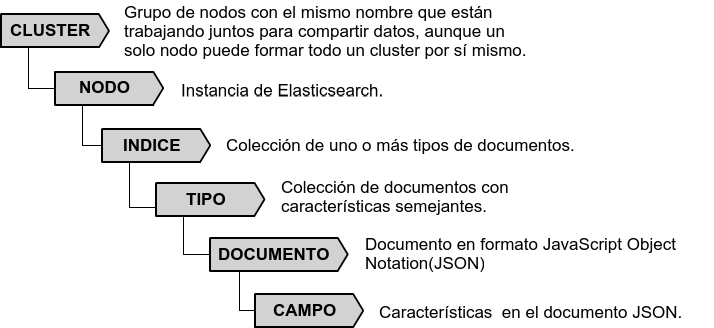
\includegraphics[height=0.26\textheight]{fig01/elastic_fields}
	\mycaption[Estructura de componentes en Elasticsearch]{Estructura de componentes en Elasticsearch.}
	\label{fig:RHP02}
\end{figure}

Como se puede observar en la Figura 2.3, Elasticsearch consta de ciertas características semejantes a las bases de datos relacionales. 

"\textit{Un cluster (grupo de nodos), puede contener múltiples índices (base de datos), cada uno contiene múltiples tipos (tablas). Estos tipos sostienen mútliples documentos (renglones), y cada documento tiene múltiples campos (columnas)"} (\citeauthor{Gormley}, \citeyear{Gormley}).

El acto de almacenamiento en Elasticsearch es llamado \textit{\textbf{Indexing}}, en donde, un índice es estructurado dentro de un nodo.  

Elasticsearch es de ''schema free'' lo cual significa que no requiere la definici\'on de un esquema, puesto que lo asigna autom\'amicamente. Para realizar la distribución de índices sobre los documentos, detecta la estructura y el tipo de datos,  e inmediatamente después hace los datos disponibles para su búsqueda y/o análisis. Asimismo, permite consultar varios índices en una sola consulta y los resultados son mostrados a una velocidad impresionante. Inclusive, Elasticseach tiene la característica de distribución masiva, sin problema alguno permite aumentar la cantidad de nodos de manera que el cluster aproveche automáticamente el hardware adicional (\citeauthor{siteElastic}, \citeyear{siteElastic}).

\textbf{\textit{Mapping}}. Proceso para definir la estructura de los datos en los documentos en Elasticsearch. Si bien Elasticsearch por default asigna un mapping automático a cada índice, existe la opción de implementar un mapping personalizado, en donde se pueden especificar ciertas propiedades de los campos dentro de la estructura del documento JSON (\citeauthor{Gormley}, \citeyear{Gormley}). 

Por ende, el almacenamiento de los documentos es realizado en base a la definición de un mapping personalizado para cada uno de los índices destinados a las fuentes de datos de interés. 

%El mapping personalizado es aplicado sobre el índice específico donde serán almacenados los documentos.

%este proceso consiste en especificar cómo serán almacenados e indexados los campos contenidos en el documento. El Mapping se utiliza para detallar el tipo de dato por campo, así como la creación de operaciones o la habilitación y deshabilitación de ciertas reglas, entre otras características.\cite{Elastic}



%==================================================%

\textbf{Etapa 5: Análisis de Datos.}
Elasticsearch analiza los documentos haciendo uso del Modelo Booleano, así como de los conceptos de frecuencia del término (tf), inversa de la frecuencia del documento (idf) y el modelo de espacio vectorial e incluye otros valores identificados como norms (\citeauthor{Gormley}, \citeyear{Gormley}).

\textit{\textbf{Modelo Booleano}}. Es el primer modelo de recuperación de información y probabilidad. Las consultas son realizadas utilizando los operadores básicos de la lógica matemática de George Boole: AND, OR y NOT, para encontrar todos los documentos que coincidan con los términos solicitados. Es usado para excluir los documentos que no coincidan con la consulta (\citeauthor{modelos_recuperacion_info}, \citeyear{modelos_recuperacion_info}).

\textit{\textbf{Frecuencia del Término / Inversa de la Frecuencia del Documento (tf/idf)}}. Es uno de los mejores modelos de recuperación de texto. La relevancia de los documentos depende del peso calculado en base a la frecuencia con la que aparece el término consultado sobre el contenido del documento.

Los documentos y la consulta pueden ser representados como un vector de frecuencia de términos \textbf{d} =  (${x_1, x_2,....,x_n}$) y \textbf{q} = (${y_1, y_2,...,y_n}$) respectivamente, donde \textit{n} es el número total de términos, ${x_i}$ y ${y_i}$ son las frecuencias del término $tf_i$ (tf) en el vector documentos (d) y el vector consulta (q), respectivamente. Dada una colección de documentos \textit{C}, la inversa de la frecuencia del documento (idf) esta definida por $log(N/n_t)$, donde \textit{N} es el número total de documentos en \textit{C}, y $n_t$ es el número de documentos que contienen el término \textit{t}. Para la representación tf/idf, todos los términos en los vectores consulta y documentos son pesados con la fórmula \textbf{d'} = ( $tf_{d(x_1)}\cdot idf_{(t_1)}, tf_{d(x_2)}\cdot idf(t_2),..., tf_{d(x_n)}\cdot idf(t_n)$) y \textbf{q'} = ( $tf_{d(y_1)}\cdot idf_{(t_1)}, tf_{d(y_2)}\cdot idf_{(t_2)},..., tf_{d(y_n)}\cdot idf_{(t_n)}$) (\citeauthor{modelo_tf_idf}, \citeyear{modelo_tf_idf}).

\textit{\textbf{Norms}}. Son una serie de características contempladas para calcular la relevancia de los documentos en Elasticsearch, tales como:
\begin{itemize}
  \item \textit{queryNorm}. Es un factor incorporado para intentar normalizar la consulta.
  \item \textit{coord}. Coordinación de la consulta. Es usada para aumentar las posibilidades de que un documento, que contiene un alto porcentaje de coincidencias con la consulta, sea más relevante que sobre otro.
  \item \textit{Field-length norm}. Contempla la longitud del campo, de manera que si el término consultado aparece en un campo corto, aumenta la probabilidad de que el contenido del campo sea sobre dicho término a que apareciera sobre un campo con mayor contenido.
  \item \textit{t.getBoost()}. Es un valor aplicado por cada término en el campo.
  
\end{itemize}

De manera, que el valor del cálculo de la relevancia de los documentos se ve afectada significativamente por el cálculo de todos estos conceptos. Por lo anterior, la implementación del mapping personalizado sobre los índices creados en Elasticsearch, permite alterar el cálculo del peso de los documentos. 

\textit{\textbf{Modelo de Espacio Vectorial}}.
Es un modelo basado en el criterio de similaridad propuesto por Gerard Salton, donde cada documento (d) y consulta (q) son representados como vectores de términos. La medida de similaridad es usualmente el ángulo del coseno en los vectores $\vec{d}$ y $\vec{q}$, proporciona un camino para comparar una consulta con múltiples términos contra un documento (\citeauthor{modelos_recuperacion_info}, \citeyear{modelos_recuperacion_info}). La fórmula está dada por: 

\begin{equation}\label{eq:Fórmula tf/idf}
score( \vec{d}, \vec{q}) = \frac{\sum_{k=1}^m {d_k}\cdot{q_k} } { \sqrt{\sum_{k=1}^m (d_k)^2} \cdot \sqrt{\sum_{k=1}^m (q_k)^2}}
\end{equation}
 
Donde el valor \textit{score} representa la similaridad entre los vectores documento ($\vec{d}$) y consulta ($\vec{q}$), calculado de la sumatoria de los productos del peso de cada documento (d) por el peso de la consulta (q), dividido sobre el producto de la raíz cuadrada de la sumatoria del cuadrado de los pesos de los documentos (d), por la raíz cuadrada de la sumatoria del cuadrado de los pesos de la consulta (q).


Los términos explicados anteriormente, son aplicados por Elasticsearch en la fórmula llamada \textit{Practical Scoring Function} utilizada para calcular la relevancia de los documentos (\citeauthor{Gormley}, \citeyear{Gormley}).
\begin{gather}
\intertext{Fórmula Practical Scoring Function}
score( q,d) = \\
queryNorm(q) \\
\cdot coord(q,d) \\
\cdot \sum{}(\\
tf(t \to\mathbb{}d) \\
\cdot idf(t)^2 \\
\cdot t.getBoost()\\
\cdot norm(t,d))
\end{gather}

\begin{gather}
(t \to\mathbb{}q)
\end{gather}

Donde: \\
(2.2)  \textit{score(q,d)} representa el valor de la relevancia de un documento (d) para la consulta (q).\\
(2.3) \textit{queryNorm(q)} es el factor de normalización.\\
(2.4) \textit{coord(q,d)} es el factor de coordinación.\\
(2.5) y (2.10) Es la sumatoria de los pesos de cada término (t) en la consulta (q) para el documento (d).\\
(2.6) \textit{tf (t$ \to\mathbb{} $d)} es la frecuencia del término (t) en el documento (d).\\
(2.7) \textit{idf (t)} es la inversa de la frecuencia del documento para el término (t).\\
(2.8) \textit{t.getBoost()} es el valor de estímulo que ha sido aplicado sobre la consulta.\\
(2.9) \textit{norm(t,d)} es la norma de la longitud del campo, combinada con el nivel del estímulo de tiempo del índice.

%==================================================%

\textbf{Etapa 6: Visualización de Datos.}
La etapa final consiste en desarrollar la interfaz de usuario, en donde puedan observarse los resultados obtenidos a las consultas solicitadas al sistema. Las tecnologías elegidas para la implementación de la interfaz fueron:

\textit{\textbf{Python}}. Es un lenguaje de programación realmente flexible, pues se adapta eficientemente a cualquier ambiente de desarrollo (\citeauthor{python}, \citeyear{python}). Fue elegido para implementar el backend del sistema SOFTSE, es decir, a través de este lenguaje los datos eran recibidos, procesados y enviados.
% * <amgdark@uaz.edu.mx> 2016-11-02T00:07:26.533Z:
%
% > Lenguaje de programación realmente flexible, pues se adapta eficientemente a cualquier ambiente de desarrollo. \cite{python} 
%
% Mencionar que se usa en el backend
%
% ^.
Entre las ventajas al utilizar Python fue que las APIs de las fuentes de datos seleccionadas, se encuentran disponibles para ser manipuladas a través de este lenguaje, permitiendo automatizar tareas como la descarga y almacenamiento de los datos.

\textit{\textbf{Django}}. Continuando con la implementación enfocada al lenguaje Python, surge la elección de Django, un framework de alto nivel para desarrollo Web en Python que trabaja bajo la arquitectura MVT (Modelo-Vista-Template) (\citeauthor{Django}, \citeyear{Django}). 
% A single figure
\begin{figure}[H]
	\centering
	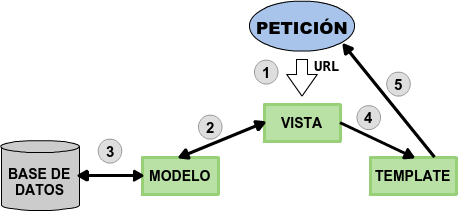
\includegraphics[height=0.23\textheight]{fig01/mvt}
	\mycaption[Arquitectura MVT Django]{Arquitectura MVT Django}
	\label{fig:RHP02}
\end{figure}

La Figura 2.4 muestra la interacción entre los componentes de la arquitectura MVT; inicia con el envío de una petición que a través de una url, dirige la solicitud hacia la vista encargada de interactuar con el modelo para obtener los datos desde la base de datos. Los datos son enviados a la vista, la cual a su vez actualiza el template con las respuestas recibidas.

\textit{Capa Modelo}.        
Capa encargada de estructurar y manipular los datos (\citeauthor{Django}, \citeyear{Django}). En nuestro caso, debido a que Elasticsearch funge como base de datos externa a Django, los modelos fueron representados a través de consultas en el lenguaje DSL\footnote{Lenguaje de consultas en formato JSON en Elasticsearch (\citeyear{dsl_elastic}).} de Elasticsearch, realizadas mediante la librería Python elasticsearch 2.3.0 (\citeauthor{apiElastic}, \citeyear{apiElastic}).
    

         % * <amgdark@uaz.edu.mx> 2016-11-02T00:08:07.342Z:
%
% >  Este paso fue sustituido por el almacenamiento de Elasticsearch.
%
% El modelo no fue sustituido, más bien los modelos se formaron a partir de consultas realizadas con elastic, favor de corregir
%
% ^.
    %  \item 
    
\textit{Capa Vista}.
En Django, la vista es representada en forma de funciones o clases Python. Es la capa responsable de la lógica de procesar y responder a las consultas de los usuarios, determina qué datos serán visualizados en el template o plantilla (\citeauthor{Django}, \citeyear{Django}).   
    
\textit{Capa Template}.        
Capa que proporciona una interfaz amigable, en donde será presentada la información al usuario (\citeauthor{Django}, \citeyear{Django}). Los recursos utilizados para diseñar el template o plantilla del sistema de búsqueda SOFTSE fueron:

Bootstrap, un popular framework para desarrollo web, implementa HTML5, CSS3 y JavaScript (jQuery), fue elegido para desarrollar el frontend (interfaz de usuario) del sistema, ya que cuenta con características que son gratamente aceptadas por los usuarios debido a los componentes que lo integran, así como la creación de una interfaz web responsiva, es decir, una interfaz que puede adaptarse a cualquier dispositivo (\citeauthor{Bootstrap}, \citeyear{Bootstrap}).

Los datos fueron estructurados a través de JavaScript, AJAX y Python, estas tecnologías permitieron realizar la manipulación de los datos recibidos a través de la capa Vista. Así como los eventos del usuario sobre el sistema.

% * <alegarcia@uaz.edu.mx> 2016-10-14T16:09:54.702Z:
%
% > Bootstrap
%
% En ésta parte estaría bien que dijeras porqué se decidieron utilizar éstas tecnologías y no otras. 
%
% ^.
%=========================================================

\chapter{Antecedentes}
\label{chap:ant}

En este capítulo, se presentan los antecedentes de investigaciones relacionadas a la problemática que se está abordando, con el objetivo de aportar mayor comprensión ante la importancia del aprovechamiento de los datos provenientes de las redes sociales, asimismo se presentan ejemplos sobre sistemas de búsqueda que basan el análisis de la información sobre los datos de los perfiles en las redes sociales.

\section{Redes sociales en Big Data}
\label{sec:sec01} 
%\initial{E}
En el mundo Big Data, las redes sociales han formado parte importante en el incremento de datos circulando por Internet. Las personas acceden a las redes sociales tanto para compartir su información como para conectarse con otras personas, produciendo un evidente aumento en la cantidad de datos. 
% * <alegarcia@uaz.edu.mx> 2016-10-24T15:26:00.712Z:
%
% > E}n el mundo Big Data, las redes sociales han formado parte importante en el incremento de datos circulando por Internet. Las personas acceden a las redes sociales tanto para compartir su información como para conectarse con otras personas, produciendo un evidente aumento en la cantidad de datos.
%
% Al final de éste párrafo, introduce lo que vas a mostrar en éste capítulo de Antecedentes, veo que dividiste los antecedentes en 2 partes, describe aquí porque están divididos en dos partes, en lo particular no me queda claro....
%
% ^.

Las redes sociales se han convertido en un campo de interés de explotación, en donde, muchos de los interesados al buscar cómo aprovechar los datos y obtener un beneficio, han realizado investigaciones con diversos intereses, tales como: el análisis de sentimientos, identificación de perfiles a tráves de su identidad, coincidencia entre perfiles de distintas redes sociales, entre otros.

\subsection{Aprovechamiento de datos en los perfiles de redes sociales}
\label{subsec:subsec01} 


\textbf{Identificación de perfiles de usuario a través de múltiples redes sociales}.
%\label{subsec:subsec01}
Generalmente, los usuarios suelen unirse a varias redes sociales, debido a que cada una tiene un enfoque en específico y  brinda distintos servicios. De manera que la información de los usuarios queda distribuida en las redes sociales a las que se unió.

Paridhi y Ponnurangam, ambos procedentes de Indraprastha Instituto de Información Tecnológica (IIIT-Delhi) en India, y Anupam de la Universidad de Maryland, USA (\citeyear{art_usersacross}), realizaron una investigación, en donde el enfoque fue mejorar un algoritmo de búsqueda tradicional basado en analizar ciertos atributos en los perfiles de usuario, y aplicarlo para encontrar el perfil de un usuario de Facebook dada su identidad en Twitter. El unir la información de varias redes sociales, en este caso de Facebook y Twitter, permitió crear la identidad de un usuario a través del complemento de la información entre las que se encuentra registrado el usuario. Esta investigación permitió tener un acercamiento hacia el \textit{matching} de los datos de los perfiles de usuario provenientes de varias redes sociales, además de mostrar los beneficios al unir más de una red social.

\textbf{Análisis de los atributos de perfiles públicos de las redes sociales}. Aunado al enfoque sobre la combinación de distintas redes sociales, el análisis de los atributos de cada uno de los perfiles de usuario es un área importante de investigación.

Bastian, Hayes, Vaughan, Shah, Skomoroch y Kim, todos pertenecientes a la Corporación de LinkedIn, realizaron una investigación sobre la funcionalidad de la sección ''Habilidades y Experiencia (Skills and Expertise)'' en la cual se destaca debido a que es un área, en donde las características que el usuario añada a su perfil, pueden ser evaluadas por los usuarios en su red de conexiones (\citeyear{art_skill_exp_link}). Si bien, la investigación se enfoca en mostrar la implementación de un sistema para sugerir características que pudiese tener el usuario, esta investigación agregó valor hacia la problemática que abordamos, ya que la coincidencia de enfocar los datos de interés sobre la misma sección destaca que es un área con gran valor dentro de los perfiles.

\textbf{Minería de datos de las redes sociales}.
La minería de datos ha sido un ámbito importante en el análisis de los datos de las redes sociales, como Twitter, Facebook, LinkedIn, Google+, cuentas de GitHub, páginas web, blogs y correos electrónicos, con el objetivo de explorar los datos y generar una solución sobre cierta problemática (\citeauthor{book_miningsocial}, \citeyear{book_miningsocial}).

Muchas investigaciones están relacionadas con la minería de datos de las redes sociales, la investigación realizada por Allamanis y Sutton, de la Escuela de Informática de la Universidad de Edinburgh, UK., en donde, la minería de datos fue aplicada sobre el código fuente de los repositorios en GitHub, con el objetivo de crear un modelo de lenguaje probabilístico de código fuente e identificar patrones conforme a la reutilización y complejidad del código (\citeauthor{art_mininggithub}, \citeyear{art_mininggithub}). De igual manera, aportó valor a la fuente de datos GitHub, que fue seleccionada pues se destaca el interés que existe por aprovechar la información de esta red social.

% * <alegarcia@uaz.edu.mx> 2016-10-24T15:29:29.063Z:
%
% > Por ello, resulta interesante, primero, elegir las redes sociales que contengan mayor cantidad de información de interés para poder dar solución a una problemática. Seguido de la identificación de los campos que serán analizados durante la búsqueda como nombre, ubicación, género, entre otros. Inclusive, las búsquedas por contenido, por menciones o publicaciones propias del usuario, o quizás, a través de la propia red de usuarios del perfil. \cite{art_usersacross}  Con el objetivo final de identificar perfiles de usuarios en base a ciertos atributos dentro de las distintas redes sociales.
%
% Ésta parte más que a antecedentes, me parece que hablas de tu metodología: elegir las redes, identificar campos, identificar perfiles etc....... Si fuera antecedentes estaría redactado diferentes: Dado que la información de los usuarios está muy dispersa en las redes sociales, se han diseñado muchas herramientas que buscan hacer matching de la información de distintas redes sociales, éstas herramientas lo que realizan es bla bla bla bla ..... eso ya suena más a antecedentes, describir lo que ya está....
%
% ^.


%================================================
\section{Sistemas de búsqueda en el ánalisis de perfiles públicos de redes sociales}
% * <alegarcia@uaz.edu.mx> 2016-10-24T15:33:00.981Z:
% 
% > Retos que resuelve el Proyecto
% Éste título causa un poco de conflicto aquí porque se trata de describir los antecedentes y no los retos de tu proyecto. Habría que cambiarlo para que describa mejor lo que quieres explicar aquí.
% 
% 
% ^.

Actualmente, existe una gran variedad de sistemas de búsqueda de perfiles en redes sociales enfocados en analizar los perfiles de usuario de una o varias redes sociales, para luego filtrarlos por nombre, alias o ubicación; también, pueden encontrarse buscadores de candidatos, los cuales realizan un análisis profundo sobre la información que proporciona el perfil, permitiendo hacer consultas específicas para filtrar los perfiles, ya sea para el ámbito laboral o personal. Desde el propio motor de búsqueda que implementa cada sitio web, buscadores tradicionales (Google, Yahoo, Bing), hasta casos como los que se describen a continuación:

\textit{YouandJob}, es un buscador de candidatos en España, parecido a Google, dirigido principalmente a las empresas que buscan posibles candidatos dentro de los perfiles registrados en este sitio (\citeauthor{youandjob}, \citeyear{youandjob}). A pesar de que las consultas son gratuitas, el sitio cuenta con algunas restricciones como contar con una cuenta y pagar 1 euro, tanto para poder ver un perfil completo como para contactar al candidato elegido; cabe mencionar que, este sitio también contaba con la opción de importar el currículum vitae desde LinkedIn por 1 euro anual, pero desafortunadamente quedó ineficaz, luego de la actualización de acceso a los datos que realizó LinkedIn en el mes de mayo del 2015. 

Asimismo, existen herramientas que fungen como complementos en ciertos sitios web, como en LinkedIn, en donde para la versión Premium dispone de una herramienta llamada \textit{LinkedIn Recruiter} (\citeauthor{linkrec}, \citeyear{linkrec}) que permite ver perfiles completos de cualquier miembro registrado y contactar con ellos mediante el complemento InMail. Cuenta con poderosas herramientas de búsqueda en LinkedIn, incluyendo una gran cantidad de filtros que facilitan la obtención de datos de un candidato específico. Como se mencionaba, es necesario tener la versión Premium (Plan: Recruiter Lite), los costos son 119.95 d\'olares mensuales o 1,119.40 dólares anuales. Otra herramienta es \textit{LinkedInTool} (\citeauthor{linktool}, \citeyear{linktool}), una herramienta fácil de usar, que consiste en copiar el link/url de la consulta avanzada realizada desde LinkedIn a LinkedInTool y con un click descarga todos los perfiles obtenidos de dicha consulta, almacenándolos en un archivo excel. Los costos del “Extractor” son 39 dólares mensuales o 380 dólares anuales. “Extractor + Connector” son 59 dólares mensuales o 500 dólares anuales. 

 
Como se puede observar, en estos casos el análisis de los datos está enfocado en examinar la propia información de la red social LinkedIn. No obstante, existen buscadores de redes sociales que nos ayudan a encontrar los perfiles de las personas que nos interesan, tales como:

\textit{Social Mention} es una plataforma de análisis y búsqueda de redes sociales, genera un resumen mostrando lo que las personas están diciendo en tiempo real sobre el tema consultado. Monitorea más de 100 redes sociales como Twitter, Facebook, FriendFeed, YouTube, Digg, Google, etc. (\citeauthor{link_socialmention}, \citeyear{link_socialmention}).

\textit{snitch.name} es una página web para encontrar a través de la consulta por nombre, los perfiles de usuario de una misma persona en una gran variedad de redes sociales (Facebook, Twitter, Linkedin, entre otros). Muestra las páginas en las que se encuentra el perfil (\citeauthor{link_snitchname}, \citeyear{link_snitchname}).

\textit{Skipease} es un buscador de personas, consta de un motor de búsqueda para cada red social, ofrece mejores resultados mientras más detalles se tengan del contacto a buscar, tales como  nombre, nombre de usuario, dirección, número de teléfono, correo electrónico u otros identificadores personales (\citeauthor{link_skipease}, \citeyear{link_skipease}).

Los ejemplos mencionados anteriormente son una pequeña muestra de la gran variedad de buscadores de redes sociales que existen, de los cuales se destaca la similitud en la búsqueda de perfiles en base a la consulta de información personal de los usuarios. De tal manera, se observa que hay pocos buscadores específicos que analicen ciertas características de los perfiles para encontrar a las personas que nos interesen. \\


% * <alegarcia@uaz.edu.mx> 2016-10-24T15:41:58.006Z:
% 
% > SOFTSE.
% Joyce, has revisado si existe alguna herramienta que haga búsquedas en GitHub ? por repositorio ? o de manera general? , si no existe mencionar que de GitHUb no encontraste alguna herramienta, y si existe describirla.... 
% 
% 
% ^.

\textbf{Metodología implementada en los sistemas de búsqueda}.
Si bien, estas soluciones podrían resolver la problemática que nos concierne, existe un punto importante, los resultados podrían cumplir o no con las expectativas del usuario en algunas ocasiones, ya que el análisis de la búsqueda de datos es realizado sobre el contenido completo de los perfiles.


Este factor, en algunas ocasiones, puede encontrarse dentro de la amplia variedad de m\'etodos y herramientas para almacenar y buscar informaci\'on, como lo son bases de datos relacionales, no relacionales o motores de b\'usqueda full-text search, ya que generalmente al realizar una consulta, el propio algoritmo de búsqueda es implementado en base al análisis de todo el contenido que se encuentra almacenado, de manera que los resultados se muestran de acuerdo a un indicador de relevancia, que es afectado por el valor de la frecuencia de las palabras coincidentes con la consulta realizada.

% * <alegarcia@uaz.edu.mx> 2016-10-28T17:10:54.352Z:
%
% > de manera que los resultados son mostrados en el orden de relevancia calculado respecto a la frecuencia obtenida del análisis.
%
% Joyce, aquí lo que quieres decir es que las herramientas actuales muestran la relevancia de acuerdo a la frecuencia en que aparecen las palabras consultadas en toodo el contenido de los documentos ? si es así trata de escribir mejor el párrafo que te señalo, "de manera que los resultados se muestran de acuerdo a un indicador de relevancia..........
%
% ^.

Sin embargo, hay casos en donde las consultas requieren ser orientadas hacia un campo espec\'ifico del documento, puesto que al determinar la relevancia de los documentos ante la frecuencia de las palabras considerando el contenido por completo, los resultados no coincidir\'an con la consulta realizada. Un ejemplo de ello es Google Search, el mejor motor de búsqueda que existe en la actualidad, que aunque el análisis de búsqueda se basa sobre 200 factores (\citeauthor{link_200google}, \citeyear{link_200google}), la relevancia de las páginas resultantes no siempre muestran la página de mayor interés para el usuario.



% * <alegarcia@uaz.edu.mx> 2016-10-24T15:50:04.291Z:
%
% > Dentro del tratamiento y an\'alisis de la informaci\'on resulta de gran inter\'es conocer la frecuencia con la que se repite una palabra o frase dentro de una colecci\'on de datos, lo anterior nos permite determinar la relevancia que tiene un documento sobre otro, y as\'i definir el orden en que ser\'an mostrados los resultados de una consulta. 
%
% Hay que redactar mejor ésto para que quede más como antecedente....... Muchas de las herramientas que existen están diseñadas para determinar la relevancia que tiene un documento respecto a....... por ejemplo..... y describes las herramientas que ya hay y que nos sirven como antecedentes !!!! Se supone que en la sección anterior de marco teórico ya explicaste lo que era relevancia, tf, idf, etc  por lo cual no sería necesario incluirlo aquí.....
%
% ^.
% * <alegarcia@uaz.edu.mx> 2016-10-24T15:47:22.548Z:
%
% > Actualmente, existe una gran variedad de m\'etodos y herramientas que permiten almacenar y buscar informaci\'on, como bases de datos relaciones, no relaciones o motores de b\'usqueda full-text search. 
%
% Como antecedentes éste párrafo que te señalé está bien......
%
% ^.
% * <alegarcia@uaz.edu.mx> 2016-10-24T15:44:16.336Z:
%
% > buscar informaci\'on
%
% buscar información en dónde ? aclarar
%
% ^.

%Por ello, a trav\'es del aprovechamiento de las caracter\'isticas del motor de b\'usqueda Elasticsearch, implementamos un mapping personalizado que permite determinar la relevancia contemplando los valores  de la frecuencia del t\'ermino de la b\'usqueda en el documento (tf) y la inversa de la frecuencia del documento (idf) sobre un campo espec\'ifico de cada documento. 

%Despu\'es de realizar la implementaci\'on de mapping sobre una colecci\'on prueba de 100 perfiles públicos de GitHub, almacenada en Elasticsearch, los resultados obtenidos mostraron que utilizando el Mapping Default, la relevancia de los documentos no coincide con el orden de los documentos que esper\'abamos, ya que el valor de tf del documento m\'as relevante no siempre es el m\'as alto. Por el contrario, al implementar nuestro Mapping Personalizado, como podemos observar en el Cuadro 3.1, el documento que muestra el valor de tf m\'as alto, presenta tambi\'en mayor peso W. Lo anterior nos permite encontrar aquellos perfiles con mayor pr\'actica en los lenguajes de programaci\'on, como respuesta a las consultas realizadas. 
% * <alegarcia@uaz.edu.mx> 2016-10-24T15:53:33.341Z:
%
% > Por ello, a trav\'es del aprovechamiento de las caracter\'isticas del motor de b\'usqueda Elasticsearch, implementamos un mapping personalizado que permite determinar la relevancia contemplando los valores  de la frecuencia del t\'ermino de la b\'usqueda en el documento (tf) y la inversa de la frecuencia del documento (idf) sobre un campo espec\'ifico de cada documento. 
% > Despu\'es de realizar la implementaci\'on de mapping sobre una colecci\'on prueba de 100 perfiles públicos de GitHub, almacenada en Elasticsearch, los resultados obtenidos mostraron que utilizando el Mapping Default, la relevancia de los documentos no coincide con el orden de los documentos que esper\'abamos, ya que el valor de tf del documento m\'as relevante no siempre es el m\'as alto. Por el contrario, al implementar nuestro Mapping Personalizado, como podemos observar en el Cuadro 3.1, el documento que muestra el valor de tf m\'as alto, presenta tambi\'en mayor peso W. Lo anterior nos permite encontrar aquellos perfiles con mayor pr\'actica en los lenguajes de programaci\'on, como respuesta a las consultas realizadas.
%
% Aquí ya estás hablando de tu herramienta, la éstas describiendo y hasta estás escribiendo resultados, esto no va aquí va en metodología, en la descripción de tu herramienta y en tus resultados..... hay que enfocarnos en antecedentes, por ejemplo el paper de LinkedIn que ya hacían extracción del campo de skills de sus usuarios, hay que mencionarlo y explicar cómo lo hicieron ellos..... y herramientas similares 
%
% ^.

%\begin{table}[H]
%\centering
%\caption{Comparaci\'on entre los resultados obtenidos sin y con mapping espec\'ifico}
%\begin{tabular}{|c|c|c|c|} 
%\hline
%\multicolumn{2}{|c|}{Mapping Default}&
%\multicolumn{2}{|c|}{Mapping Personalizado}\\
%\hline
%TF&W&TF&W\\ \hline
%5& 1.0598&221&239.42 \\ \hline
%9&1.0156&193&209.0926\\ \hline
%6&0.9951&135&146.2565\\ \hline
%135&0.9834&125&135.4227\\
%\hline\end{tabular}
%\end{table}

%\subsection{Escalabilidad de las búsquedas específicas y otros sectores}

%En una primera instancia el sistema fue enfocado en buscar perfiles públicos a través de consultas de habilidades dentro del sector de Ingeniería de Software y conocimientos sobre lenguajes de programación. Pero, es importante mencionar que la búsqueda del sistema puede ser extendida a otros campos del perfil de los usuarios o se puede ampliar a otros sectores diferentes al de Ingenieria de Software.
% * <alegarcia@uaz.edu.mx> 2016-10-24T15:56:42.320Z:
%
% > En una primera instancia el sistema fue enfocado en buscar perfiles públicos a través de consultas de habilidades dentro del sector de Ingeniería de Software y conocimientos sobre lenguajes de programación. Pero, es importante mencionar que la búsqueda del sistema puede ser extendida a otros campos del perfil de los usuarios o se puede ampliar a otros sectores diferentes al de Ingenieria de Software.
%
% Éste párrafo va al final del capítulo de resultados.... al mencionar que tu herramienta es escalable a otros campos y a otros sectores...... 
%
% Éste párrafo va al final del capítulo de resultados.... al mencionar que tu herramienta es escalable a otros campos y a otros sectores...... 
%
% ^.

%====================================


Aunado a lo anterior, y debido a la poca existencia en la explotación de datos implementados en sistemas de búsqueda específicos para encontrar perfiles públicos enfocados en el sector de Ingeniería de Software, se decidió implementar SOFTSE.
% * <alegarcia@uaz.edu.mx> 2016-10-24T15:57:47.649Z:
%
% > Como se puede observar, los ejemplos mencionados anteriormente se centrar en perfiles provenientes de LinkedIn, ya que ésta es una de las fuentes de datos elegidas para implementar nuestra solución. Si bien, estas soluciones podrían resolver nuestra problemática, existe un punto importante, el análisis de la búsqueda de datos es realizado sobre el contenido completo de los perfiles, lo cual genera resultados que contemplan tanto la cercanía o relación con mis contactos, como el análisis del contenido.
% > Aunado a lo anterior, y dedibo a la poca existencia en la explotación de datos implementados en sistemas de búsqueda específicos para encontrar perfiles públicos enfocados en el sector de Ingeniería de Software,se decidió implementar SOFTSE.
%
% Éstos párrafos están bien para finalizar el capítulo de antecedentes, así déjalos....... 
%
% ^.





%=========================================================

\chapter{Metodología del proyecto}
\label{chap:enf}

Anteriormente, en el Capítulo 2 fueron descritas cada una de las etapas propias del Modelo de Proceso de Análisis definido para llevar a cabo el desarrollo del proyecto. En este capítulo, son detallados los procedimientos y herramientas implementados durante cada etapa del proceso de análisis, en el desarrollo del sistema de búsqueda de perfiles públicos llamado \textit{SOFTSE}

\section{Proceso de análisis.}
\label{sec:sec04}



\subsection{Selección de fuentes de datos.}
\label{subsec:subsec04}

Haciendo referencia al Capítulo 2, en donde las fuentes de datos seleccionadas fueron: la red social para profesionales llamada LinkedIn,  la plataforma de desarrollo colaborativo GitHub (\citeyear{fields_github}) y la red social Twitter (\citeyear{fields_twitter}), pues se determinó que éstas administran datos de interés ante nuestra propuesta de solución, y están relacionadas con perfiles públicos involucrados en el sector de Ingenier\'ia de Software. 

\textbf{Datos administrados en las fuentes de datos seleccionadas.}
A continuación se muestra la mayor cantidad de información relevante en este trabajo, que es manipulada por las fuentes de datos: GitHub, LinkedIn y Twitter. De esta manera, al evaluar la información que es administrada en cada una de estas redes sociales,  se pueden determinar los campos que abarcan la información de interés para la búsqueda y análisis de los perfiles de usuario, proporcionando información suficiente al interesado al momento de elegir un candidato óptimo a sus necesidades.

\renewcommand{\tablename}{Tabla}

%\setlength{\parindent}{0.5cm}

\begin{table}[H] %\textit{\textbf{Datos en los perfiles de LinkedIn.}} \\
\centering
\begin{tabular}{|p{5cm} p{9cm}|}
\hline
\textbf{Campo} & \textbf{Descripción} \\
\hline \hline
Nombre & Nombre y apellidos\\ 
\hline
Titular profesional & Puesto actual de trabajo.\\
\hline
Ubicación & \\
\hline
Sector & Enfoque laboral\\
\hline
Información de contacto & {Correo electrónico, teléfono, sitios web.}\\
\hline
Extracto & Información sobre objetivos, logros y metas.\\
\hline
Experiencia & Experiencia profesional incluidos empleos, puestos de voluntario, en el ejército, en consejos de administración, y en organizaciones sin ánimo de lucro o deportivas profesionales.\\
\hline
Educación & Información universitaria y educativa.\\
\hline
Recomendaciones & Recomendaciones profesionales realizadas por otros. \\
\hline
Certificaciones & Certificaciones, licencias o permisos que ha obtenido.\\
\hline
Cursos & Cursos principales que ha realizado.\\
\hline
Reconocimientos y premios & Premios que ha obtenido con esfuerzo.\\
\hline
Idiomas & Idiomas que entiende o habla.\\
\hline
Organizaciones & Organizaciones o asociaciones a las que ha pertenecido, así como el cargo que desempeñó.\\
\hline
Patentes & Cualquier patente que haya solicitado o adquirido.\\
\hline
Publicaciones & Publicaciones que demuestran su trabajo.\\
\hline
Proyectos & Proyectos en los que ha trabajado, así como los miembros de los equipos.\\
\hline
Aptitudes y validaciones & Lista de aptitudes.\\
\hline
Calificaciones de pruebas & Notas de calificaciones destacadas obtenidas en los exámenes.\\
\hline
Experiencia de voluntario y causas benéficas &  Organizaciones que apoya, causas que le interesan y los tipos de oportunidades de voluntariado que busca.\\
\hline
Información adicional & Intereses, datos personales como fecha de nacimiento o estado civil, e información de otros medios de contacto.\\
\hline
\end{tabular}
\caption[Campos administrados en LinkedIn]{Algunos campos del perfil LinkedIn (\citeyear{fields_link}).}
\label{tabla:Campos LinkedIn}
\end{table}

%=========================
\begin{table}[H]
    \centering
    \begin{tabular}{|p{5cm} p{9cm}|}
    \hline
    \textbf{Campo} & \textbf{Descripción} \\
    \hline \hline
	Nombre & Nombre Completo o Alias.  \\
    \hline

	Correo Electrónico Público & \\
    \hline

	URL & Alojar pequeños sitios web desde repositorios públicos en GitHub. Formato: http://username.github.io.\\
    \hline
	
    Compañía/Empresa & \\
	\hline
    Ubicación & \\
   \hline
   Repositorios & Lista de repositorios públicos especificados por el usuario.\\
   \hline


    \end{tabular}
    
\caption[Campos administrados en GitHub]{Algunos campos del perfil GitHub (\citeyear{fields_github}).}
\label{tabla:Campos GitHub}
\end{table}
%======================================
 \begin{table}[H]
    \centering
    \begin{tabular}{|p{5cm} p{9cm}|}
    \hline
    \textbf{Campo} & \textbf{Descripción} \\
    \hline \hline
    Nombre & Nombre y apellidos\\ 
    \hline
    Ubicación & \\
    \hline
    Tweet & Contenido del tweet publicado\\
    \hline
	Fecha de Tweet & Fecha y horario de publicación. \\
    \hline
    \end{tabular}
\caption[Campos administrados en Twitter]{Algunos campos del perfil Twitter (\citeyear{fields_twitter}).}
\label{tabla:Campos Twitter}
\end{table}

%\begin{itemize}
       % \item       
        %\item \textit{\textbf{Datos en los perfiles de GitHub}}. 
     

%\item \textit{\textbf{Datos en los perfiles de Twitter}}.
    
%\end{itemize}



%\begin{table}[H]
%\begin{center}
%\begin{tabular}{|l|l|}
%\hline
%\textbf{Campo} & \textbf{Descripción}\\
%\hline
%Aptitudes y validaciones & Lista de aptitudes.\\
%\hline
%\end{tabular}
%\caption{Listado de alumnos}
%\end{center}
%\end{table}




%las fuentes de datos seleccionadas fueron: la red social para profesionales llamada LinkedIn, la red social Twitter y la plataforma de desarrollo colaborativo GitHub, pues se determinó que administran datos que son de interés ante nuestra propuesta de solución, además se encuentran relacionados con perfiles públicos involucrados en el sector de Ingenier\'ia de Software. 


De la información presentada en las Tablas 4.1, 4.2 y 4.3, fueron seleccionados aquellos campos que contienen datos de interés ante la solución propuesta, dicha información puede observarse en la Figura 4.1. \\

%A figures matrix.
\begin{figure}[H]
\centering
\begin{minipage}{3.3cm}
    \centering
    \subtop[]{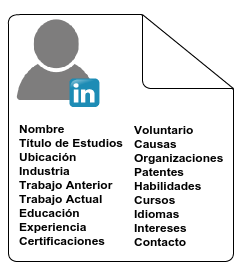
\includegraphics[height=0.22\textheight]{fig01/linkedin_data}\label{sf:multiRH02a}}
\end{minipage}
\hspace{1.2cm}
\begin{minipage}{3.3cm}
    \centering
    \subtop[]{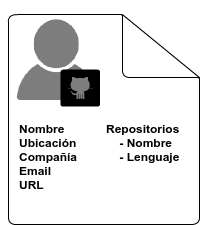
\includegraphics[height=0.2\textheight]{fig01/github_data}\label{sf:multiRH02b}}
\end{minipage}
\hspace{0.7cm}
\begin{minipage}{3.3cm}
    \centering
    \subtop[]{
\includegraphics[height=0.18\textheight]{fig01/twitter_data}\label{sf:multiRH02c}}
\end{minipage}


%\\ \vspace{0.1cm}
%\begin{minipage}{10cm}
   % \centering
    %\subtop[]%{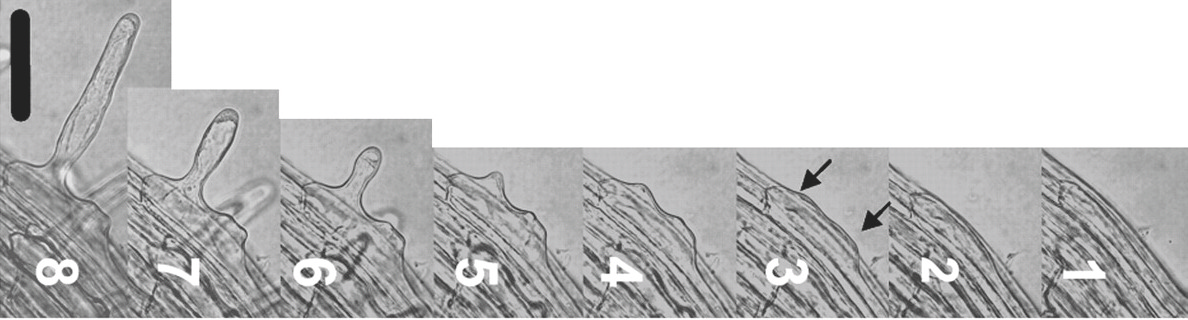
\includegraphics[height=0.145\textheight]{fig01/mutantrhd6}\label{sf:multiRH02d}}
%\end{minipage}
%\\ \vspace{0.1cm}
%\begin{minipage}{10cm}
 %   \centering
%    \subtop[]%{\includegraphics[height=0.16\textheight]%{fig01/auxab}\label{sf:multiRH02e}}
%\end{minipage}

%\mycaption[Hair-forming mutant cells.]{(a) A mutant RH cell. Asterisks show multiple sites of RH initiation in a single root hair cell (indicated by the arrows). Figure reproduced from \cite{}. (b)~Hair-forming cell with three RH initiation locations. The bar represents $50\mu m$. Figure reproduced from \cite{}. (c) Large bump in mutant {\itshape rhd1}. Figure reproduced from \cite{}. (d) Mutant overexpressing gene {\itshape ROP2}; from right-hand to left-hand, numbers indicate progressive snapshots at different times. RH initiation sites are indicated by the arrows. The bar represents $75\mu m$. Figure reproduced from~\cite{}. (e)~Mutants affected by auxin. On the left-hand side, RH site is farther away from the apical end (left arrow cap); on the right-hand side, multiple RH locations (arrows). Figure reproduced from~\cite{}.}
\mycaption[Datos seleccionados de los perfiles públicos]{ Datos seleccionados en los perfiles de las redes sociales de: (a) LinkedIn , (b) GitHub y (c) Twitter.}
\label{fig:multiRH02}
\end{figure}

Como se puede observar, los datos provenientes de LinkedIn se enfocan en proporcionar informaci\'on te\'orica de los candidatos que tiene que ver con la experiencia laboral, conocimientos, habilidades, entre otros datos. GitHub, se concentra en almacenar proyectos de desarrollo de software y provee los datos prácticos de los perfiles de usuario, por ejemplo, los conocimientos sobre ciertos lenguajes de programación. Al unir la información de las dos redes sociales, nos permite obtener información más precisa y fidedigna de una gran cantidad de perfiles de usuario en cuanto a su experiencia.

Aunado a lo anterior, se decide incluir Twitter pues a través de microblogs nombrados tweets, se puede obtener información reciente sobre lo que la gente está hablando. Para el caso de SOFTSE, los tweets mostrados son en base a los términos consultados relacionados con experiencia y habilidades en el área de Ingeniería de Software.

 %++++++++++++++++++++++++++++++++++++++++++++++++++++++
 % Book mining social web 
% http://www.webpages.uidaho.edu/~stevel/504/Mining-the-Social-Web-2nd-Edition.pdf
% http://plg.math.uwaterloo.ca/~migod/papers/2014/msr14-Oleksii-ElasticSearch.pdf
% http://homepages.inf.ed.ac.uk/csutton/publications/msr2013.pdf
% https://www.diva-portal.org/smash/get/diva2:638844/FULLTEXT01.pdf
 
%+++++++++++++++++++++++++++++++++++++++++++++++++++++++++
 
%========================================================

\subsection{Extracción de datos.}
\label{subsec:subsec04}

La etapa de extracción de datos requirió el uso de varios recursos tales como las APIs disponibles en las redes sociales seleccionadas, así como distintas técnicas para extraer los datos de interés en este trabajo. A continuación, son descritos los procedimientos aplicados para cada una de las fuentes de datos.

\textit{\textbf{GitHub y Python}}. 
La extracción de datos en GitHub, fue realizada a través de la disposición del API propia de la plataforma colaborativa, y la manipulación de ésta por medio de la librería de Python llamada PyGithub versión 1.29 (\citeauthor{pygithub}, \citeyear{pygithub}). Con lo anterior, fue diseñado un script encargado de automatizar el proceso de autenticación y extracción de los datos.

El proceso inicial para accesar al API de Github consiste en enviar las claves de autenticación obtenidas, en este caso, se utilizaron las llaves OAuth2 Key/Secret, ya que permiten realizar mayor cantidad de solicitudes sobre el API.

Dentro del script, las llaves de autenticación son enviadas a través de una instancia (g) de Github, propia de la librería PyGithub, tal como se muestra en la siguiente instrucción: \texttt{g = Github(''llave\_cliente", "llave\_secreta")}

El acceso a los datos es a través de una instancia de Github (g), de manera que para obtener los perfiles públicos se utiliza la instrucción: \texttt{g.get\_users()}, en donde, los datos de interés obtenidos de cada perfil son: nombre, ubicación, compañía, email y un conjunto de repositorios; dentro de cada repositorio se obtiene nombre, descripción, lenguaje de programación y url del repositorio. Los campos descritos anteriormente, son extraídos, estructurados y almacenados en documentos JSON (Figura 4.2).

% A single figure
\begin{figure}[H]
	\centering
	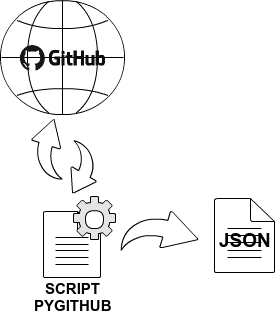
\includegraphics[height=0.22\textheight]{fig01/extraccion_git}
	\mycaption[Extracción de datos en GitHub]{Extracción de datos en GitHub.}
	\label{fig:RHP02}
\end{figure}

El script fue ejecutado continuamente, puesto que al llegar al límite de peticiones (5,000 solicitudes por hora), éste era “dormido” por 5 minutos y regresaba a realizar peticiones. 

\textbf{X-Raying Google - LinkedIn}. 
A causa de que el API de LinkedIn sufrió actualizaciones de restricción de acceso a los datos, se opta por utilizar la técnica llamada X-Raying utilizando el motor de búsqueda Google.

% A single figure
\begin{figure}[H]
	\centering
	
\includegraphics[height=0.18\textheight]{fig01/extraccion_link}
	\mycaption[Extracción de datos en LinkedIn]{Extracción de datos en LinkedIn.}
	\label{fig:RHP02}
\end{figure}

Como se observa en la Figura 4.3, a través de consultas como: \textit{site:mx.linkedin.com/in “ingeniero de software”}. En donde, los perfiles son filtrados en primera instancia por el título de \textit{ingeniero de software}, puesto que es el enfoque de nuestra solución. Desafortunadamente, con la limitante de resultados mostrados en el motor de búsqueda Google, se opta por tomar la decisión de filtrar los perfiles por países. De manera que se obtuvieron un aproximado de 1000 perfiles de ingenieros de software provenientes de los países de Argentina, Brasil, Canadá, México y Estados Unidos.


Una vez realizada la consulta sobre el motor de búsqueda Google, por cada uno de los perfiles, la información es capturada y estructurada en documentos JSON, para después ser pre-procesados.


\textbf{Logstash y Elasticsearch - Twitter}. 
La recolección de tweets consistió en el procesamiento de logs, a través de la combinación de Logstash y Elasticsearch. Inicialmente, para llevar a cabo este proceso, es requerido la autorización de acceso al API de Twitter, la cual se obtiene mediante las llaves de autenticación (Consumer Key, Consumer Secret, Access Token y Access Token Secret), además son requeridas las coordenadas de la zona que será analizada.


% A single figure
\begin{figure}[H]
	\centering
	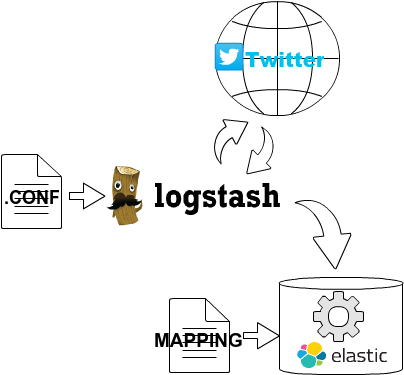
\includegraphics[height=0.24\textheight]{fig01/extraccion_tweet}
	\mycaption[Extracción de tweets]{Extracción de tweets.}
	\label{fig:RHP02}
\end{figure}

Una vez recopilados los datos, el proceso a seguir  como se observa en la Figura 4.4, consiste en crear un archivo de configuración (.conf) dentro de la carpeta bin en Logstash, este archivo contendrá las instrucciones específicas para la extracción de la información, es el encargado de enviar las llaves de acceso al API de Twitter y solicitar los datos de los perfiles. El propio archivo de configuración se encarga de almacenar los perfiles obtenidos en Elasticsearch. En la Figura 4.5, se muestra un ejemplo del contenido del archivo.

% A single figure
\begin{figure}[H]
	\centering
	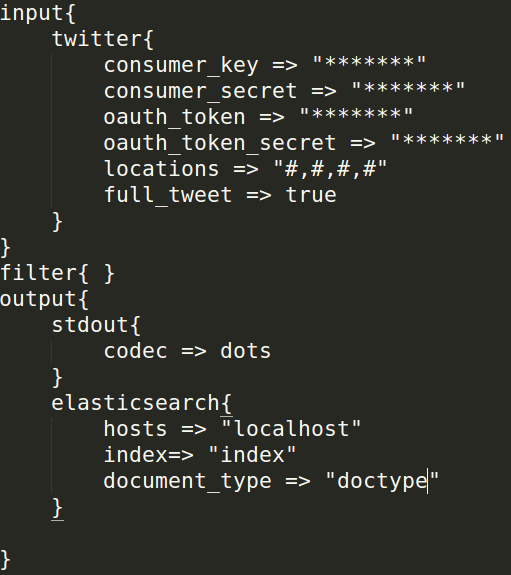
\includegraphics[height=0.25\textheight]{fig01/twitter_conf}
	\mycaption[Archivo de configuración para recolectar tweets]{Archivo de configuración para recolectar tweets.}
	\label{fig:RHP02}
\end{figure}

Luego de establecer el archivo de configuración en Logstash, se crea un nuevo índice en Elasticsearch, el cual requiere la definición del esquema mapping para distribuir los datos durante la descarga.

% A single figure
\begin{figure}[H]
	\centering
	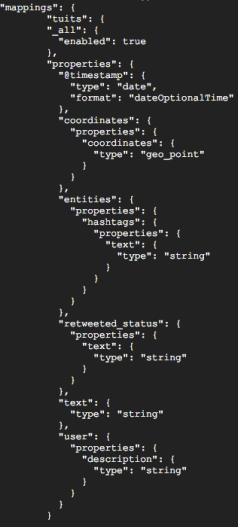
\includegraphics[height=0.47\textheight]{fig01/recolector_mapp}
	\mycaption[Creación de un nuevo índice para tweets]{Creación de un nuevo índice con tipo de documento y mapping de la información recolectada de los tweets.}
	\label{fig:RHP02}
\end{figure}

La Figura 4.6 muestra un ejemplo de esquema mapping, el cual sigue la estructura de datos provenientes de Twitter. Una vez configurado el esquema sobre el índice donde serán almacenados los datos de los tweets, se procede a iniciar la recolección de los tweets; nos dirigimos a la dirección donde fue creado el archivo de configuración, e iniciamos la ejecución mediante la instrucción:
\textit{\$ ./logstash -f file.conf}

Cabe destacar que el proceso para la recolección de datos mencionado anteriormente, fue logrado gracias a las instrucciones publicadas por Coronado (\citeyear{recolector_tweets}).

%=======================================================
\subsection{Pre-Procesamiento de Datos}
\label{subsec:subsec04}

Después de definir los campos a estructurar, a través de la creación de un script los datos fueron pre-procesados, de manera que las inconcistencias de los datos son eliminadas, para luego establecerlos sobre las estructuras mapping. Entre las inconsistencias observadas, se encontraron caracteres como tabulador, diagonales invertidas (\textbackslash{}), valores inexistentes, tildes (\textasciitilde{}), entre otras.

%======================================================%
\subsection{Almacenamiento de Datos}
\label{subsec:subsec04}

A partir de la definición y limpieza de los campos a estructurar, procedemos a establecer el esquema de mapeo o mapping para los índices enfocados en almacenar los datos de LinkedIn y GitHub. Es importante mencionar que un mapping debe ser incluido durante la creación de un índice.

% A single figure
\begin{figure}[H]
	\centering
	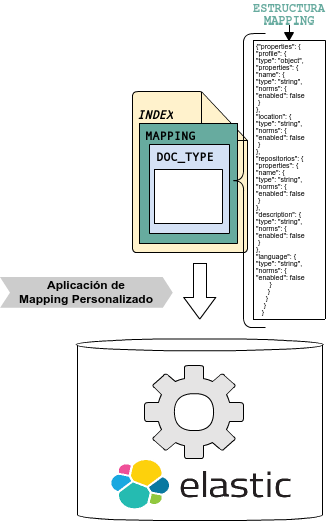
\includegraphics[height=0.325\textheight]{fig01/apply_mapping}
	\mycaption[Proceso de implementación mapping]{Proceso de implementación mapping personalizado}
	\label{fig:RHP02}
\end{figure}


La Figura 4.7, muestra el proceso para el mapeo de campos seleccionados, que consiste en la creación de un índice (\_index)\footnote{Colección de documentos que tienen algo en común (\citeauthor{elastic_meta}, \citeyear{elastic_meta}).}, asignado al tipo de documento (\_type)\footnote{Clase del objeto designada para representar el documento (\citeauthor{elastic_meta}, \citeyear{elastic_meta}).}, que es afectado a través de las propiedades definidas para el mapping de los datos. Como se menciona en el Capítulo 2, la relevancia de los documentos es determinada en base a tres factores: tf, idf y norms, siendo este último factor (norms), un valor con gran impacto sobre el peso calculado en los documentos, pues al evaluar aspectos como la longitud de los campos y complementándolo con otros factores, pudiesen ser de valor, en caso que el análisis  requiriera procesar el contenido completo de los documentos. Caso contrario al que nos concierne, pues el análisis de los documentos está dirigido a procesar sólo los campos que contienen los datos de interés. De manera que se opta por deshabilitar los cálculos norms mediante la esquematización mapping, teniendo como resultado documentos evaluados utilizando únicamente el modelo tf/idf.

% A single figure
\begin{figure}[H]
	\centering
	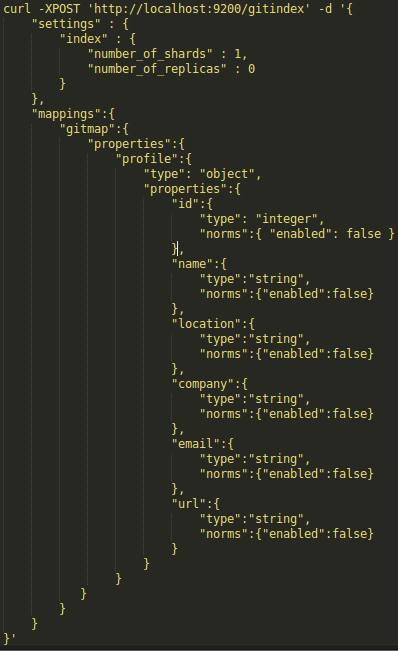
\includegraphics[height=0.4\textheight]{fig01/mappgit}
	\mycaption[Estableciendo mapping]{Estableciendo mapping.}
	\label{fig:RHP02}
\end{figure}
En la Figura 4.8, se puede observar un ejemplo de esquematización mapping, aplicada sobre el índice creado llamado \textit{gitindex} con un tipo de documento \textit{gitmap}. De tal manera, que muestra la definición de los campos a estructurar y la deshabilitación de las \textit{norms} por cada campo.


%==================================================%

\subsection{Análisis de Datos}
\label{subsec:subsec04}

Luego de aplicar las configuraciones sobre los índices de almacenamiento, el análisis de los datos, ahora es dirigido a examinar los conjuntos de datos relevantes, donde se encuentran almacenados los datos de interés para nuestra solución.

Continuando con la información del ejemplo anterior (gitindex), el proceso de análisis de datos es aplicado sobre el dato de interés \textit{lenguaje\_de\_programacion}, que forma parte de los campos pertenecientes a los elementos del subconjunto de \textit{repositorios} en los perfiles de GitHub. 

% A single figure
\begin{figure}[H]
	\centering
	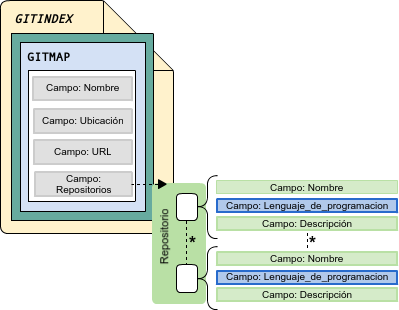
\includegraphics[height=0.25\textheight]{fig01/mapping_g}
	\mycaption[Identificación de campos de interés a analizar]{Ejemplo de identificación de los campos de interés a analizar}
	\label{fig:RHP02}
\end{figure}

Como se puede observar en la Figura 4.9, el campo lenguaje\_de\_programacion, resaltado en color azul, contiene la información a analizar. Debido a que
% Tal es el caso de los perfiles de GitHub, en donde el dato de interés \textit{lenguaje\_de\_progra- macion}, forma parte de los campos pertenecientes a los elementos contenidos en el subconjunto de \textit{repositorios} en los perfiles. 
%De manera que, como se muestra en el punto 4 de la Figura 4.8, se requiere accesar directamente al subconjunto que contiene los datos de interés.
%Lo anterior puede suceder gracias a que
Elasticsearch permite realizar búsquedas específicas a través de consultas por campos (\citeauthor{Gormley}, \citeyear{Gormley}), para analizar el campo \textit{lenguaje\_de\_programacion} en el subconjunto \textit{repositorios}, se realiza una consulta semejante a la siguiente:
{\small \textit{ localhost:9200/gitindex/gitmap/\_search? q=perfil.repositorios.lenguage\_de\_programacion:texto\_de\_busqueda}}, indicando la dirección del servidor, seguido del nombre del índice (gitindex) destinado para almacenar los documentos (gitmap) al que fueron definidos. La última instrucción indica la dirección donde se encuentra el campo de interés para el análisis. 

De modo que al dirigir el análisis de los datos sobre el campo de lenguaje\_de\_programa- cion, el cálculo de la relevancia de los documentos es afectado, únicamente, por la frecuencia de los términos coincididos sobre ese campo. 

Cabe mencionar, que este proceso fue aplicado tanto en los perfiles de GitHub y LinkedIn, únicamente difiriendo en el campo de análisis.


% A single figure
%\begin{figure}[H]
%	\centering
%	\includegraphics[height=0.3\textheight]%{fig01/procesomappingv1}
%	\mycaption[Proceso de implementación mapping]{Proceso de implementación mapping personalizado en Elasticsearch: 1) Mapping, 2) Extracción de Datos, 3) Almacenamiento, 4) Consultas por campo}
%	\label{fig:RHP02}
%\end{figure}

% * <alegarcia@uaz.edu.mx> 2016-11-22T16:44:07.961Z:
%
% En el poster de Chihuahua te quedó muy bien ilustrado todo el proceso, mi recomendación es que aquí lo cambies y lo dejes como lo tienes en el poster, y te extiendas un poco más en la explicación de cada etapa del proceso. 
%
% ^.
%==================================================%

\subsection{Visualización de Datos}
\label{subsec:subsec04}

Cumpliendo con la estructura de la arquitectura MVT implementado por Django, cada una de las etapas fue aplicada como se muestra a continuación (Figura 4.10):

% A single figure
\begin{figure}[H]
	\centering
	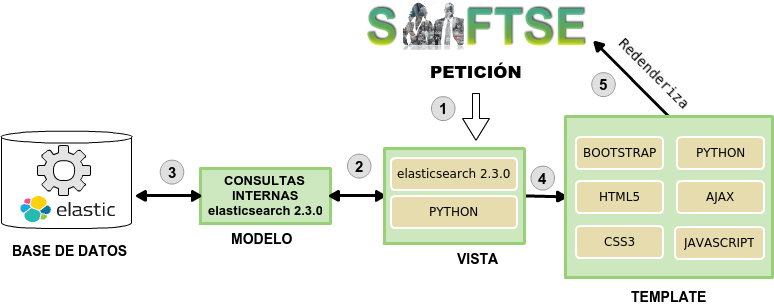
\includegraphics[height=0.24\textheight]{fig01/mvt_process}
	\mycaption[Arquitectura MVT Django en SOFTSE]{Arquitectura MVT Django en SOFTSE}
	\label{fig:RHP02}
\end{figure}

En la Figura 4.10 se puede observar las tecnologías empleadas en cada una de las capas de la arquitectura MVT de Django, además se muestra la interacción entre éstas; donde por medio de la interfaz de SOFTSE, la petición es ejecutada y enviada hacia la vista encargada de solicitar los datos al modelo. Los datos son enviados a la vista, la cual a su vez renderiza el template con las respuestas recibidas.


\textbf{Capa Modelo}. Los modelos fueron representados por consultas DSL realizadas en código Python a Elasticsearch (base de datos externa a Django) por medio de la librería Python \textit{elasticsearch 2.3.0}. La Figura 4.11, muestra un ejemplo del formato DSL en que son realizadas las consultas hacia Elasticsearch, dentro de la cual se especifican el índice (index) al que accesará y el tipo de documento (doc\_type) al que fueron asignados los documentos de los perfiles. Como se puede observar, el cuerpo de la consulta (body) consiste en una cadena de instrucciones indicando el tipo de búsqueda que será realizada; en este caso la consulta definida es \textit{match}, ya que se requiere encontrar los perfiles que coincidan con la información enviada.

% A single figure
\begin{figure}[H]
	\centering
	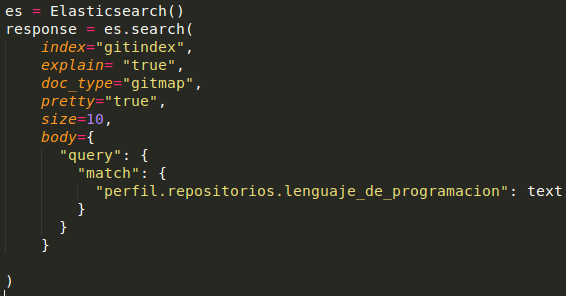
\includegraphics[height=0.2\textheight]{fig01/dsl_query}
	\mycaption[Consulta DSL a Elasticsearch]{Ejemplo de consulta DSL a Elasticsearch}
	\label{fig:RHP02}
\end{figure}



%\item 
\textbf{Capa Vista}.
Las vistas (funciones) están definidas para procesar las respuestas a las consultas DSL recibidas de los modelos. Los datos son evaluados y preparados, de tal manera que cumplan las estructuras que serán recibidas y procesadas para mostrar la información destinada a la interfaz de usuario.

%\item 
\textbf{Capa Template}.
El frontend del sistema SOFTSE, fue desarrollado utilizando los lenguajes de HTLM5 y CSS3 para dar formato a la interfaz. Debido a que esta capa se encarga de distribuir los datos recibidos de las vistas, se recurrió a emplear los lenguajes de programación Python, JavaScript y AJAX, embebidos sobre HTML5. 

De manera que Python fungió como el administrador de la información consultada y enviada por las vistas. Tanto JavaScript como AJAX fueron utilizados para implementar la reacción a los eventos recibidos en la interfaz de usuario, como clickear un botón o un enlace, por ejemplo. Si bien, JavaScript por si sólo puede cumplir estas tareas, AJAX fue requerido por motivos de pérdida de información durante el proceso de consultas, ya que, una vez que la primer consulta era realizada, al necesitar hacer otras consultas, los datos no alcanzaban a ser recuperados durante la actualización de la página, y por ende, eran perdidos. 

% A single figure
\begin{figure}[H]
	\centering
	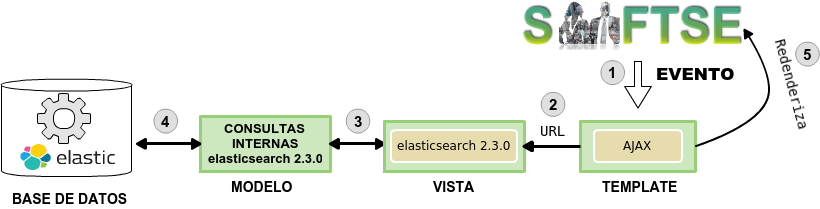
\includegraphics[height=0.17\textheight]{fig01/proceso_ajax}
	\mycaption[Proceso de AJAX en Django]{Proceso de AJAX en Django}
	\label{fig:RHP02}
\end{figure}

En la Figura 4.12, puede observarse el proceso de consultas empleando AJAX, que al no requerir actualizar la página para enviar y recibir datos, dio solución a la pérdida de los datos que se presentaba. El proceso implementado entre AJAX en Django, consiste inicialmente en recibir un evento sobre la interfaz de usuario, que está definida por funciones AJAX encargadas de hacer las peticiones a la vista para realizar las consultas a la base de datos y enviar la respuesta a la función AJAX que reaccionó al evento; finalmente, la función distribuye los datos recibidos en la interfaz de usuario.

 
% * <alegarcia@uaz.edu.mx> 2016-11-07T17:11:16.843Z:
%
% > nto JavaScript como AJAX fueron destinados para reaccionar a los eventos dentro de la interfaz como clickear un botón o recargar la página, aunque AJAX reacciona a los eventos en la interfaz sin la necesidad de recargar la página para no perder la información mostrada.
%
% Aquí me causa un poco de confusión, se seleccionó JavaScript y AJAX para reaccionar a eventos o recargar página, pero después dices que AJAX reacciona sin recargar la página porque se puede perder la información, entonces me confundí un poco, es necesario recargar la página ? lo hacemos? o no lo hacemos?, creo que es cosa de redacción para que lo cheques sale. 
%
% ^.


%\end{itemize}

 

%=========================================================

\chapter{Sistema SOFTSE}
\label{chap:softse}

\initial{S}\textit{OFTSE} (Software Skills and Experience) es un sistema de búsqueda para encontrar perfiles públicos involucrados en el área de Ingeniería de Software, a través del análisis de los perfiles pertenecientes a la red social de profesionales LinkedIn y a la plataforma colaborativa GitHub. SOFTSE está diseñado para recibir consultas relacionadas con habilidades de Ingenieros de Software y conocimientos sobre lenguajes de programación. El objetivo principal es agilizar el proceso de búsqueda de perfiles, y está dirigido a todo aquel que requiera encontrar un candidato involucrado en el área de Ingeniería de Software.

% A single figure
\begin{figure}[H]
	\centering
	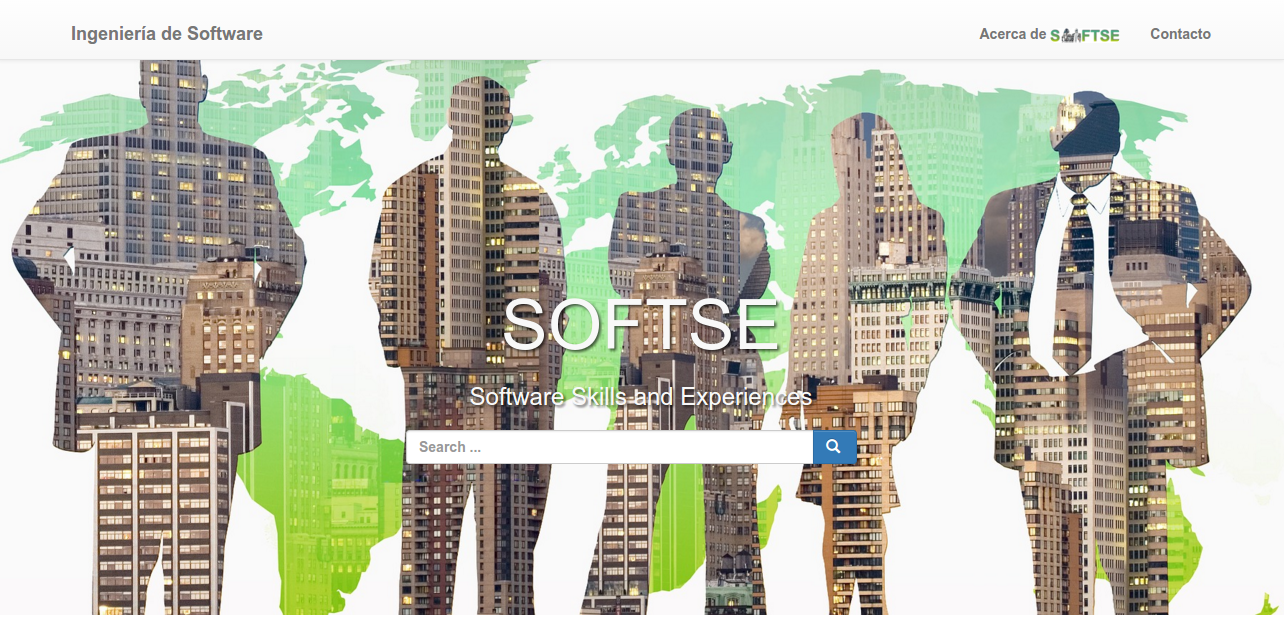
\includegraphics[height=0.2\textheight]{fig01/softse_1.png}
	\mycaption[Página principal del sistema SOFTSE]{Página principal del sistema SOFTSE}
	\label{fig:RHP02}
\end{figure}

Como se observa en la Figura 5.1, SOFTSE consta de un campo de texto en donde el interesado ingresa la consulta; una vez realizada la solicitud, los perfiles públicos coincidentes a la consulta son mostrados sobre dos secciones: \textit{LinkedIn} y \textit{GitHub}, respectivamente. Asimismo, existe una sección llamada \textit{News} que muestra los tweets publicados en tiempo real por los usuarios pertenecientes a Twitter.

\section{Descripción de las secciones}
\label{sec:sec05}

Las secciones de LinkedIn y GitHub contienen una lista de perfiles públicos, dividida en pequeñas páginas, cada una con un máximo de 5 perfiles.

\textbf{LinkedIn}. En esta sección son mostrados los perfiles públicos de LinkedIn, en donde la consulta es analizada sobre el campo de habilidades, permitiendo encontrar aquellos candidatos que muestran tener conocimientos relacionados con los términos solicitados. 

%A figures matrix.
\begin{figure}[H]
\centering
\begin{minipage}{3.3cm}
    \centering
    \subtop[]{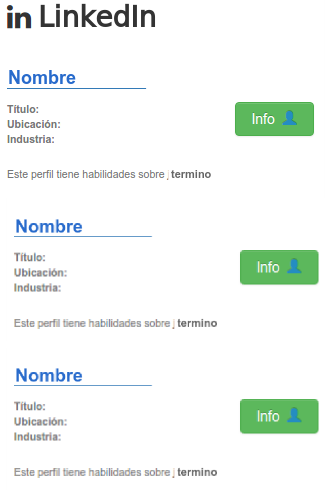
\includegraphics[height=0.35\textheight]{fig01/secLinked}\label{sf:multiRH02a}}
\end{minipage}
\hspace{2cm}
\begin{minipage}{3.3cm}
    \centering
    \subtop[]{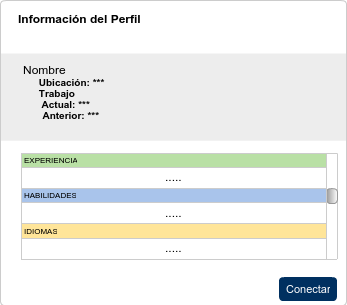
\includegraphics[height=0.2\textheight]{fig01/perfilLinked}\label{sf:multiRH02b}}
\end{minipage}

\mycaption[Sección LinkedIn]{ Sección de LinkedIn: (a) Lista de perfiles encontrados, (b) Información por perfil}
\label{fig:multiRH02}
\end{figure}

La Figura 5.2 (a) muestra el diseño de la interfaz de usuario de cómo son mostrados los datos de los perfiles obtenidos de la consulta. Cada uno de los elementos mostrados en la lista pertenece a un perfil público, de manera que en primer instancia sólo aparecen los datos básicos del perfil, como nombre, ubicación, industria o lugar donde labora y el título o nivel académico. Asimismo, fue agregada una pequeña leyenda que indica que el perfil tiene las habilidades que fueron consultadas por el interesado.

En caso que algún perfil sea atractivo para el interesado, éste puede recurrir a ver más información del perfil (Figura 5.2 (b)), de tal manera que pueda determinar si es o no el candidato que buscaba, y hacer contacto a través de la propia red social LinkedIn.


\textbf{GitHub}.
Esta sección muestra los perfiles públicos de GitHub en donde la consulta se enfoca en el análisis sobre el campo \textit{lenguaje \_de\_programacion}, que pertenece a cada uno de los repositorios de cada perfil. 

%A figures matrix.
\begin{figure}[H]
\centering
\begin{minipage}{3.3cm}
    \centering
    \subtop[]{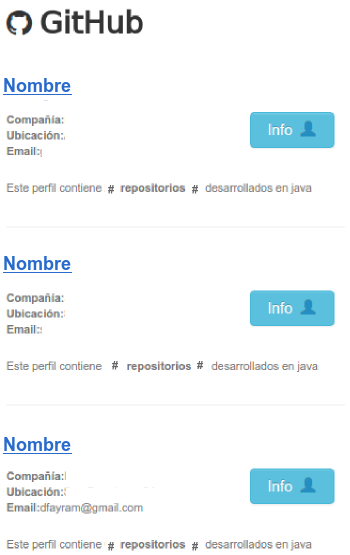
\includegraphics[height=0.35\textheight]{fig01/secGithub}\label{sf:multiRH02a}}
\end{minipage}
\hspace{2cm}
\begin{minipage}{3.3cm}
    \centering
    \subtop[]{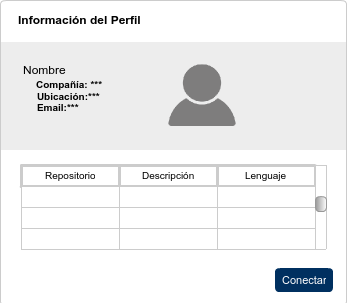
\includegraphics[height=0.2\textheight]{fig01/perfilGit}\label{sf:multiRH02b}}
\end{minipage}

\mycaption[Sección GitHub]{ Sección de GitHub: (a) Lista de perfiles encontrados, (b) Información por perfil}
\label{fig:multiRH02}
\end{figure}

Al igual que en la sección \textit{LinkedIn}, los perfiles obtenidos de la consulta aparecen sobre una lista de elementos ordenados de manera descendente, en donde el primer perfil es aquel que contiene la mayor cantidad de repositorios desarrollados en los lenguajes de programación coincidentes a la consulta. De igual manera, cada elemento incluye la información básica de cada perfil como nombre, compañía, ubicación y correo electrónico (email), además de una breve leyenda que indica la cantidad de repositorios que contiene el perfil, así como el número de repositorios coincidentes con los términos solicitados.

La Figura 5.3 (b) muestra la información complementaria al perfil, dentro del cual incluye la información básica, además la información sobre los repositorios desde el nombre del repositorio, la descripción y el lenguaje de programación en que fue desarrollado.


\textbf{News}.
Una vez realizada la consulta, esta sección muestra los tweets filtrados por la búsqueda enfocada en el contenido del mensaje. Tiene la finalidad de mantener informado al interesado acerca de lo que las personas están hablando sobre los términos consultados.

% A single figure
\begin{figure}[H]
	\centering
	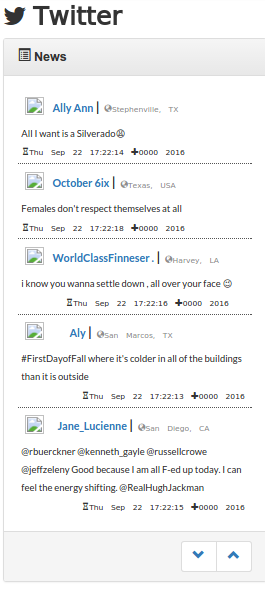
\includegraphics[height=0.58\textheight]{fig01/secTwitter.png}
	\mycaption[Sección News]{Sección News}
	\label{fig:RHP02}
\end{figure}

Como se muestra en la Figura 5.4, cada uno de los tweets mostrados incluyen el nombre de usuario del perfil, la ubicación, el contenido del tweet, así como la fecha y horario en que fue publicado.
% * <alegarcia@uaz.edu.mx> 2016-11-22T16:46:55.350Z:
%
% También mejorar la figura 5.4, el tamaño de las letras es pequeño !!
%
% ^.
%=========================================================

\chapter{Evaluación y resultados}
\label{chap:resul}

Este capítulo presenta las medidas de evaluación empleadas para determinar la efectividad del sistema SOFTSE en la recuperación de información; la evaluación del sistema fue aplicada sobre una muestra representativa.  


\section{Medidas de evaluación SRI.}
\label{sec:sec06}

Existen una amplia variedad de criterios utilizados para evaluar los sistemas de recuperación de información (SRI), tales como: “la cobertura de una colección; el tiempo de respuesta del sistema; la forma de presentación de los resultados; el esfuerzo realizado por el usuario; la exhaustividad y la precisión del sistema” (\citeauthor{RIJ}, \citeyear{RIJ}). de los cuales sólo se contemplan aquellos relacionados con el enfoque de evaluación.
Dependiendo del enfoque de la evaluación son considerados los criterios a evaluar.

%https://digitum.um.es/xmlui/bitstream/10201/4316/1/libro-ri.PDF***

%https://www.upf.edu/hipertextnet/numero-1/evaluacion_ri.html ***

%http://andresmarketing.blogspot.mx/2012/02/calculo-del-tamano-de-muestra-optimo.html

%https://books.google.com.mx/books?id=-_gr5l3LbpIC&pg=PA62&dq=calculo+del+tama%C3%B1o+muestral&hl=es-419&sa=X&ved=0ahUKEwi5g9GdgcPQAhVCwYMKHabBCLIQ6AEIGzAA#v=onepage&q=calculo%20del%20tama%C3%B1o%20muestral&f=false

%http://www.eumed.net/libros-gratis/2006a/cag2/19.htm

\subsection{Evaluación basada en la relevancia de documentos.}
\label{subsec:subsec06}

Para este trabajo de tesis, el enfoque de evaluación fue dirigido en la relevancia de los documentos.
Antes de comenzar con las medidas de evaluación, es importante definir el concepto de \textit{relevancia}, pues será la base para determinar la eficiencia de las medidas obtenidas. 

Según el Diccionario de la Real Académia, el concepto \textit{relevancia} significa ''calidad o condición de relevante; importancia, significación''. Sin embargo, es una definición de poca ayuda, pues al aplicar la relevancia sobre los documentos, surge la controversia entre los autores al determinar cuándo un documento es relevante o no. Por ello, recurrimos en la definición de Martínez (\citeyear{book_RI}), quien define un documento relevante como: ''un documento que aporte algún contenido relacionado con nuestra petición, refiriéndonos al punto de vista del usuario final que realiza una operación de recuperación de información''. 

\textbf{Medidas basadas en la relevancia.} Luego de determinar la relevancia de los documentos, procedemos a explicar los cuatro posibles resultados, que son comprendidos en las medidas de evaluación de los SRI.

\begin{table}[H]
    \centering
    \begin{tabular}{|p{4cm} p{4cm} p{4cm}|}
    \hline
 	 & \textbf{Correctos} & \textbf{Incorrectos} \\
    \hline \hline
    \textbf{Recuperados} & True Positive (TP) & False Positive (FP)\\
    \hline
\textbf{No recuperados} & False Negative (FN) & True Negative (TN)\\
    \hline
    \end{tabular}
\caption[Métricas de precisión y exahustividad]{Métricas de precisión y exahustividad (\citeauthor{tesis_evaluacion}, \citeyear{tesis_evaluacion}).}
\label{tabla:metricas de evaluacion}
\end{table}

Partiendo del conjunto de documentos \textbf{recuperados}, como se muestra en la Tabla 6.1, podemos determinar dos grupos: los \textit{documentos relevantes recuperados (TP)} que son aquellos correctamente recuperados, y los \textit{no relevantes (FP)} que fueron recuperados por error. Sin embargo, existe otro grupo de documentos, los \textbf{no recuperados}, que a su vez se dividen en: \textit{relevantes (TN)} que por error de lógica no fueron recuperados, y los \textit{no relevantes (FN)} que fueron rechazados correctamente.

\begin{align*}
\intertext{\textbf{\textit{Precisión}.} Mide el porcentaje de los documentos correctamente recuperados (TP) sobre el total de de la colección de los documentos recuperados, que está dado por la suma de los documentos relevantes recuperados (TP) y los documentos erróneamente recuperados (FP).}\\
precisión = \frac{TP}{(TP+FP)}
\end{align*}

Esta medida sirve para determinar el nivel de precisión de los documentos que fueron recuperados. Cuanto más se acerque el valor de la precisión a 1, menor será la cantidad de documentos recuperados.


\begin{align*}
\intertext{\textbf{\textit{Exhaustividad}.} Mide el procentaje de los documentos relevantes recuperados (TP) del total de los documentos relevantes, independientemente, hayan o no sido recuperados.}
exhaustividad = \frac{TP}{(TP+FN)}
\end{align*}

La definición de esta medida puede resultar un poco confusa, ya que para determinar el valor de exhaustividad, previamente es requerido conocer la cantidad total de documentos relevantes presentes en la colección. 

%En nuestro caso, al no contar con dicha información se opta por evalúar la recuperación de información del sistema, mediante la métrica de precisión.

%https://digitum.um.es/xmlui/bitstream/10201/4316/1/libro-ri.PDF
%https://www.upf.edu/hipertextnet/numero-1/evaluacion_ri.html

%  \begin{table}[H]
%     \centering
%     \begin{tabular}{|p{5cm} p{9cm}|}
%     \hline
%     \multicolumn{2}{|c|}{\textbf{Medidas basadas en la relevancia} } \\    
%     \hline \hline
%     Precisión & Documentos relevantes recuperados divididos entre el total de documentos recuperados. \\
%     \hline
% Exhaustividad & Documentos relevantes recuperados dividido entre el total de documentos relevantes. \\ 
% 	\hline
% Promedio de la efectividad E-P & Promedios de la efectividad en pares de valores de exhaustividad y precisión. \\
%     \hline
%     \end{tabular}
% \caption[Medidas basadas en la relevancia]{Medidas basadas en la relevancia (\citeauthor{book_medidas}, \citeyear{bookhttps://www.upf.edu/hipertextnet/numero-1/evaluacion_ri.html_medidas}).}
% \label{tabla:Campos Twitter}
% \end{table}

\textbf{Experimento de evaluación.} La base de datos del sistema SOFTSE está compuesta aproximadamente de 50,000 perfiles de GitHub y 4,900 perfiles de LinkedIn, por ello, se decidió tomar una muestra representativa en ambos casos, y evaluar el nivel de precisión en la recuperación de información desempeñada en el sistema.

Con el objetivo de analizar el comportamiento del sistema de búsqueda, el experimento fue aplicado sobre una muestra del uno porciento (1\%) del total de los perfiles de LinkedIn y GitHub. La evaluación fue realizada sobre la información recuperada de las consultas de términos individuales y compuestos.

El experimento consistió en buscar los términos de búsqueda por separado y obtener la cantidad de documentos que los contienen. A partir de ello, se hizo la búsqueda con las distintas combinaciones entre los términos. Cabe mencionar que tanto para el caso de GitHub como LinkedIn, el experimento fué aplicado utilizando los términos de búsqueda \textit{Ruby} y \textit{Java}.

\textit{\textbf{Evaluación en GitHub.}} Tal y como se mencionó anteriormente, el primer paso fue realizar la búsqueda de cada término sobre la colección de los documentos almacenados, obteniendo de esta manera los valores de 421 y 139 para los términos Ruby y Java respectivamente, cantidades de los documentos que indicaron presentar el término consultado. Después las búsquedas fueron ejecutadas para las posibles combinaciones entre los términos, en este caso puesto que sólo se utilizaron dos términos habrán dos combinaciones: \textit{Ruby \& Java} y \textit{Java \& Ruby}. 

La siguiente tabla muestra los valores obtenidos al aplicar cada una de las combinaciones sobre la búsqueda; en el primer caso (Ruby \& Java) se puede observar un porcentaje del 100\% de precisión y exhaustividad sobre la búsqueda del término Ruby, al recuperar exactamente los 421 documentos relevantes (TP) sin ningún documento recuperado por error (NP) o faltante (FN). En cambio para el término Java, el porcentaje de exhaustividad continúa siendo del 100\% pero el porcentaje de precisión disminuye a 93\%, ésto al recuperar 10 documentos por error (NP) además de los 139 documentos relevantes (TP). 

El segundo caso (Java \& Ruby) muestra cómo se invirtieron los papeles al obtener un porcentaje de precisión y exhaustividad del 100\% sobre el término Java y un porcentaje de precisión del 99\% en el término Ruby pues se recuperó un documento erróneo (FP) además de los 421 documentos relevantes (TP).  \\

\begin{center}
\begin{table}[H] 
\centering
\begin{tabular}{|p{3cm} p{2cm} p{2cm} p{2cm} p{2cm}|}
\hline
& \multicolumn{2}{c}{\textbf{Ruby \& Java}} & \multicolumn{2}{c|}{\textbf{Java \& Ruby}} \\ \hline
 & Ruby & Java & Java & Ruby \\
\hline \hline 
\textbf{TP} & 421 & 139 & 139 & 421 \\ \hline
\textbf{NP} & 0 & 10  & 0 & 1 \\ \hline
\textbf{FN} & 421 & 139  & 139 & 421 \\ \hline
\textbf{Precisión} & 1 & 0.93 & 1 & 0.99\\ \hline
\textbf{Exhaustividad} & 1 & 1  & 1 & 1 \\ \hline
\end{tabular}
\caption{Resultados de la precisión en GitHub}
\label{tabla:Tabla de Resultados}
\end{table}
\end{center}

\textit{\textbf{Evaluación en LinkedIn.}} La Tabla 6.3 muestra los resultados obtenidos de la evaluación aplicada a los documentos de LinkedIn con los mismos casos de prueba utilizados en la evaluación de GitHub, donde se determinaron los valores de 2 y 26 en las cantidades de documentos que contienen los términos Ruby y Java respectivamente.

El primer caso (Ruby \& Java) muestra un porcentaje del 100\% de precisión y exhaustividad sobre la búsqueda del término Ruby, al recuperar únicamente los 2 documentos relevantes (TP) dentro de la colección. En cambio para el término Java, el porcentaje de exhaustividad continúa siendo del 100\% pero el porcentaje de precisión disminuye a 93\%, ya que además de recuperar los 26 documentos relevantes (TP) fueron recuperados 2 documentos por error (NP), 

En el segundo caso (Java \& Ruby) se puede observar que el porcentaje de precisión y exhaustividad es del 100\% sobre ambos términos, ésto indica que el sistema recuperó exactamente los documentos relevantes a la consulta.

\begin{center}
\begin{table}[H] 
\centering
\begin{tabular}{|p{3cm} p{2cm} p{2cm} p{2cm} p{2cm}|}
\hline
& \multicolumn{2}{c}{\textbf{Ruby \& Java}} & \multicolumn{2}{c|}{\textbf{Java \& Ruby}} \\ \hline
 & Ruby & Java & Java & Ruby \\
\hline \hline 
\textbf{TP} & 2 & 26 & 26 & 2 \\ \hline
\textbf{NP} & 0 & 2  & 0 & 0 \\ \hline
\textbf{FN} & 2 & 26  & 26 & 2 \\ \hline
\textbf{Precisión} & 1 & 0.93 & 1 & 1\\ \hline
\textbf{Exhaustividad} & 1 & 1  & 1 & 1 \\ \hline
\end{tabular}
\caption{Resultados de la precisión en LinkedIn}
\label{tabla:Tabla de Resultados}
\end{table}
\end{center}

%======================================================

\chapter{Conclusiones y Trabajo Futuro}
\label{chap:conytf}

Dentro del contexto de Big Data, este trabajo de tesis propone un sistema de búsqueda de perfiles involucrados en el sector de Ingeniería de Software, aprovechando la información de los usuarios de redes sociales que administran datos que son de interés para nuestro caso.

La definición del modelo de análisis de datos, formó parte esencial en la implementación del sistema, ya que durante cada una de las etapas del modelo, se logró experimentar con distintas estrategias tanto para la extracción, como para el almacenamiento y procesamiento de los datos.

Asimismo, se pudo percibir cómo los propietarios de ciertos sitios web han limitado el acceso de los datos, al descubrir el gran valor que éstos proporcionan.

El trabajar con enormes cantidades de datos requiere de tecnologías destinadas para ello, tal fue el caso de Elasticsearch, un poderoso motor de búsqueda de texto \textit{full-text search}, que además de soportar el almacenamiento de grandes cantidades de información, y  la especificación de un esquema llamado \textit{mapping personalizado}, permitió tomar el control del cálculo de la relevancia de los documentos, facilitanto el filtro de los documentos de acuerdo al campo de inter\'es de las consultas para el sistema.

\textbf{Trabajo Futuro}.
En primera instancia, el sistema fue enfocado en analizar perfiles públicos a través de consultas de habilidades dentro del sector de Ingeniería de Software y conocimientos sobre lenguajes de programación. Pero es importante mencionar que la búsqueda del sistema se puede ampliar al análisis de otros campos de interés en los perfiles de usuario. Inclusive, podría ampliarse o cambiarse por completo el sector de investigación, distinto del sector de Ingeniería de Software. Lo anterior debido a que actualmente existe una gran necesidad por aprovechar y localizar perfiles de usuario tanto para fines personales, académicos, laborales, relaciones networking, entre otros.

Es importante mencionar que el sistema en su version actual está limitado a analizar los perfiles de LinkedIn que fueron almacenados durante el proceso, debido a la restricción de acceso en los datos que se enfrentó. Por ello, explorar en un futuro el procesamiento de los perfiles en tiempo real puede aumentar el impacto del sistema al recuperar la información reciente de los perfiles.

A partir de la experiencia trabajando con Elasticsearch, se propone como trabajo futuro, aplicar la implementación del mapping personalizado sobre diferentes redes sociales para realizar an\'alisis de comportamiento de usuarios en redes sociales, an\'alisis de sentimientos y de textos en sitios web considerando campos espec\'ificos.
